 %18.9.03

\chapter{Euler-Charakteristik und Perkolationsschwellen}
\label{sec:schranken}

Nachdem wir in den vorangehenden Kapiteln Methoden vorgestellt haben, mit denen die mittlere Euler-Charakteristik f\"ur Perkolationsprozesse auf Gittern berechnet werden kann, werden im Folgenden die Euler-Charakter\-ist\-iken einer Vielzahl zwei- und dreidimensionaler Gitter bestimmt. Die Resultate liefern weitere empirische Best\"atigung f\"ur die in der Einleitung vorgestellten Beobachtungen. Dar\"uberhinaus unterst\"utzen Skalenargumente die Vermutung, dass f\"ur zweidimensionale Gitter die Nullstelle $p_0$ der Euler-Charakteristik \"uber der Perkolationsschwelle $p_c$ liegt, falls $p_c>\frac{1}{2}$ ist, und dass $p_0<p_c$ ist, falls $p_c<\frac{1}{2}$ ist. Mit der in Kapitel \ref{sec:mixed} beschriebenen Methode kann die Euler-Charakteristik f\"ur bond-site-Perkolation berechnet werden, und die Beziehung zwischen der Nullstelle der Euler-Charakteristik und der Perkolationsschwelle auf bond-site-Perkolation erweitert werden.


\section{Euler-Charakteristiken in zwei Dimensionen}

Die Perkolationsschwelle $p_c$ archimedischer Gitter (siehe Abschnitt \ref{sec:archilattices}) ist kleiner als die Nullstelle $p_0$ und gr\"o"ser als der Wendepunkt $p_0^{(2)}$ der mittleren Euler-Charakteristik. Das arithmetische Mittel aus $p_0$ und $p_0^{(2)}$ liefert eine exzellente Approximation von $p_c$. Die Ergebnisse der Untersuchung weiterer zweidimensionaler Gitter best\"atigen dieses Verhalten; f\"ur $p_c<\frac{1}{2}$ kehren sich beide Ungleichungen um und man findet $p_0<p_c<p_0^{(2)}$. Allerdings gibt es auch Gitter, f\"ur die diese Ungleichungen nicht gelten. Auf diese Gitter wird im Kapitel \ref{sec:grenzen} genauer eingegangen.

\subsection{Laves-Gitter}
Laves-Gitter sind die dualen Gitter der archimedischen Gitter \cite{Gruenbaum:86}. Da archimedische Gitter nur einen Vertextyp haben, sind alle Plaketten der Laves-Gitter gleich. Die Kantenzahl der Plaketten ist die Koordinationszahl $z$ des archimedischen Gitters. Wie im Kapitel \ref{sec:chimittel} beschrieben, betrachten wir die unabh\"angige Besetzung der Plaketten der archimedischen Gitter mit Wahrscheinlichkeit $q=1-p$. Im Folgenden beziehen sich die Begriffe Plaketten, Ecken und Kanten auf die archimedischen Gitter mit Vertexkonfiguration $(n_1,\ldots,n_z)$ (siehe Kapitel \ref{sec:archilattices}). Die Euler-Charakteristik l\"asst sich am einfachsten \"uber die Beitr\"age disjunkter Zellen berechnen. Dazu bestimmen wir die erwartete Anzahl der offenen Plaketten, der randlosen Kanten und der Ecken, die bei Besetzung der Vertices mit abgeschlossenen Plaketten bedeckt werden.
\begin{itemize}
\item Die \textbf{Plaketten} sind mit Wahrscheinlichkeit $q$ bedeckt.
\item Jede \textbf{Ecke} ist von $z$ Plaketten umgeben; diese Plaketten haben $n_i$ Ecken, $i=1\ldots,z$. Daher besteht zwischen der Zahl der Ecken $E$ und der Zahl der Plaketten $F$ die Beziehung  $F=E \sum_{i=1}^z \frac{1}{n_i}$. Eine Ecke ist bedeckt, wenn mindestens eine der umgebenden Plaketten besetzt ist, und daher mit Wahrscheinlichkeit $1-(1-q)^z=1-p^z$ vorhanden. Die erwartete Anzahl der bedeckten Ecken pro Plakette ist $\frac{1-p^z}{\sum_{i=1}^z \frac{1}{n_i}}$.
\item Da jede \textbf{Kante} an zwei Ecken endet, und von jeder Ecke $z$ Kanten ausgehen, gilt f\"ur die Zahl der Kanten $K$ und Ecken $E$ die Relation $2K=zE$. Eine Kante ist bedeckt, wenn mindestens eine der angrenzenden Zellen besetzt ist, und daher mit Wahrscheinlichkeit $1-(1-q)^2=1-p^2$ vorhanden. F\"ur die erwartete Anzahl der bedeckten Kanten pro Plakette erh\"alt man $\frac{z(1-p^2)}{2\sum_{i=1}^z \frac{1}{n_i}}$.
\end{itemize}
Mit diesen Gr\"o"sen ist die mittlere Euler-Charakteristik pro Vertex 
\begin{equation}
    \bar{\chi}(q) = q- \frac{z}{2 \sum_{i=1}^z \frac{1}{n_i}}(1-p^2)+\frac{1}{\sum_{i=1}^z \frac{1}{n_i}}(1-p^z).
\end{equation}
Die Euler-Charakteristik ist von der Reihenfolge, in der die Polygone um die Vertices angeordnet sind, unabh\"angig. Dar\"uberhinaus gilt f\"ur einen planaren, zusammenh\"angenden Graphen nach dem Euler'schen Satz $F-E+V=1$. Daraus erh\"alt man
\begin{equation}
  F\left(1-\frac{z}{2 \sum_{i=1}^z \frac{1}{n_i}}+\frac{1}{\sum_{i=1}^z \frac{1}{n_i}}\right)=1
\end{equation}
und weiter unter Vernachl\"assigung von Termen $\sim 1/F$ die Beziehung $\sum_{i=1}^z \frac{1}{n_i}=\frac{z}{2}-1$. Die Euler-Charakteristiken der dualen archimedischen Gitter h\"angen also nur von der Koordinationszahl $z$ der archimedischen Gitter ab:
\begin{equation}
 \bar{\chi}(q) =q-\frac{z}{z-2}(1-p^2)+\frac{2}{z-2}(1-p^z).
\end{equation}
Die Euler-Charakteristik des Komplements ist  
\begin{equation}
\fbox{$ \displaystyle
   \chi(p) =-\bar{\chi}(q)=p(1-p)\left( 1-\frac{2}{z-2}\sum_{i=1}^{z-2}p^{i}\right).$
}
\end{equation}
Die site-Perkolationsschwellen der Laves-Gitter sind, wo sie nicht exakt oder als archimedische Gitter bekannt sind, von van der Marck \cite{Marck:03} numerisch bestimmt worden. Die Ergebnisse sind in Tabelle \ref{tab:laves} zusammengefasst. Einen Plot der Daten findet man in Abbildung \ref{fig:2dallplots}. F\"ur Laves-Gitter gilt wie f\"ur archimedische Gitter $p_0^{(2)}\leq p_c \leq p_0$. Die Korrelation von $p_0$ und $p_0^{(2)}$ mit $p_c$ ist aber nicht so bemerkenswert gut wie bei den archimedischen Gittern. Die Euler-Charakteristik der Laves-Gitter h\"angt nur von der Kantenzahl der Plaketten des Gitters ab; die Perkolationsschwellen der Gitter, deren Plaketten gleich viele Kanten haben, sind aber i. A. unterschiedlich.

\begin{table}[tb]
\centering
\begin{tabular}{|l|l||r|r|r||r|}
\hline
Duales (archimedisches) Gitter & $\frac{\chi(p)}{p(1-p)}$ & $p_0$ & $p_0^{(2)}$&$\frac{p_0+p_0^{(2)}}{2}$&$p_c$  \\ \hline
\hline

$3,12^2$ &$1-2p$&$1/2$ & $1/2$&$1/2$&$1/2$\\ \hline
 
$4,6,12$ &$1-2p$&$1/2$ & $1/2$&$1/2$&$1/2$\\ \hline

$4,8^2$&$1-2p$&$1/2$ & $1/2$&$1/2$&$1/2$\\ \hline

$6^3$, Sechseckgitter &$1-2p$&$1/2 $ & $1/2$&$1/2$&$1/2$\\ \hline

$3,6,3,6$, Kagom\'egitter&$1-p-p^2$&$0.6180$ & $0.5774$&$0.5977$&$0.5848(2)$ \\ \hline

$3,4,6,4$ &$1-p-p^2$&$0.6180$ & $0.5774$&$0.5977$&$0.5824(2)$ \\ \hline

$4^4$, Quadratgitter&$1-p-p^2$&$0.6180$ & $0.5774$&$0.5977$&$0.5927$ \\ \hline

$3^4,6$ &$1-\frac{2(p+p^2+p^3)}{3}$&$0.6914$ & $0.6300$&$0.6607$& $0.6396(2)$ \\ \hline

$3^2,4,3,4$ &$1-\frac{2(p+p^2+p^3)}{3}$&$0.6914$ & $0.6300$&$0.6607$&$0.6500(2)$  \\ \hline

$3^3,4^2$ &$1-\frac{2(p+p^2+p^3)}{3}$&$0.6914$& $0.6300$&$0.6607$&$0.6476(2)$  \\ \hline

$3^6$, Dreiecksgitter&$1-\frac{p+p^2+p^3+p^4}{2} $&$0.7413$ & $0.6687$&$0.7050$&$0.6970(2)$ \\ \hline

 \hline

\end{tabular}
\caption{Die mittleren Euler-Charakteristiken der Laves-Gitter: Die erste Spalte enth\"alt die Vertexkonfigurationen der dualen archimedischen Gitter. Die zweite Spalte enth\"alt die reduzierte Euler-Charakteristik $\frac{\chi(p)}{p(1-p)}$ der Laves Gitter. In den folgenden Spalten sind die Nullstellen $p_0$ und die Wendepunkte $p_0^{(2)}$ von $\chi(p)$, sowie $\frac{p_0+p_0^{(2)}}{2}$ angegeben. In der letzten Spalte stehen die site-Perkolationsschwellen $p_c$ der Laves-Gitter. Die ersten vier Gitter bestehen nur aus Dreiecken; daher ist $p_c=\frac{1}{2}$. Die \"ubrigen Perkolationsschwellen, abgesehen vom Quadratgitter, wurden in \cite{Marck:03} numerisch bestimmt. Die Perkolationsschwelle des Quadratgitters stammt aus \cite{Suding:99}.}
\label{tab:laves}
\end{table}

\subsection{2-uniforme Gitter}
\label{sec:2-uniform}
Es liegt nahe, als Verallgemeinerung der archimedischen Gitter mit einem Vertextyp, entsprechende Gitter mit zwei unterschiedlichen Vertextypen zu betrachten. 2-uniforme Gitter sind Gitter aus regelm\"a"sigen Polygonen gleicher Kantenl\"ange und zwei verschiedenen Vertextypen (siehe \cite{Gruenbaum:86}). Es gibt genau 20 verschiedene 2-uniforme Gitter (siehe Abbildungen im Abschnitt \ref{sec:numerik2-uniform}). Diese Gitter lassen sich, analog zu den archimedischen Gittern, durch ihre Vertextypen charakterisieren. Jeder Vertextyp $\nu$ wird durch die Folge $(n_1,\ldots,n_{z_\nu})_{\nu}$ der Kantenzahlen $n_i$ der Polygone, die den Vertex umgeben, beschrieben. Dar\"uberhinaus ist der Anteil $s_\nu$ eines Vertextyps an der Gesamtzahl der Vertices zur Unterscheidung der Gitter wichtig. Bis auf die Gitter 18 und 19 (siehe \ref{sec:numerik2-uniform}) sind so alle Gitter eindeutig bezeichnet. Die Euler-Charakteristik eines Gitters ist durch $(n_1,\ldots,n_{z_\nu})_{\nu}$ und $s_\nu$ vollst\"andig festgelegt.\\
Um die Euler-Charakteristik zu berechnen, bestimmen wir die Zahlen der bedeckten Kanten und Ecken des dualen Gitters, wenn duale Plaketten mit Wahrscheinlichkeit $q=1-p$ besetzt werden. 
\begin{itemize}
\item Jedem Vertex entspricht eine duale \textbf{Plakette}, die mit Wahrscheinlichkeit $q$ besetzt ist. 
\item Zu jeder Kante des 2-uniformen Gitters gibt es eine duale \textbf{Kante}. Die mittlere Koordinationszahl des 2-uniformen Gitters ist $\bar{z}=s_1z_1+s_2z_2$. Daher ist die Zahl der Kanten pro dualer Plakette $\frac{\bar{z}}{2}$.  Die Kanten sind mit Wahrscheinlichkeit $1-p^2$ bedeckt und die erwartete Anzahl bedeckter Kanten pro dualer Plakette ist $\frac{\bar{z}(1-p^2)}{2}$.
\item Zu einem Vertex des Typs $\nu$ des 2-uniformen Gitter ``geh\"ort'' $1/n_{i}(\nu)$ der ihn umgebenden Plaketten mit Kantenzahl $n_{i}(\nu)$, $i=1,\ldots,z_\nu$. Jeder dieser Plaketten entspricht eine \textbf{Ecke} des dualen Gitter, die mit Wahrscheinlichkeit $1-p^{n_{i}(\nu)}$ bedeckt ist. Um die erwartete Anzahl der Ecken pro dualer Plakette zu bestimmen, muss man \"uber beide Vertextypen und alle die Vertices umgebenden Plaketten summieren, und erh\"alt $\sum_{\nu=1,2}\sum_{i=1}^{z_\nu}\frac{s_\nu}{n_{i}(\nu)}(1-p^{n_{i}(\nu)})$.  
\end{itemize}
F\"ur die Euler-Charakteristik ergibt sich dann:
\begin{equation}
  \bar{\chi}(q)=q-\frac{\bar{z}}{2}(1-p^2)+\sum_{\nu=1,2}\sum_{i=1}^{z_\nu}\frac{s_\nu}{n_{i}(\nu)}(1-p^{n_{i}(\nu)}).
\end{equation}
Hiervon kann ein Faktor $p(1-p)$ abgespalten werden und man erh\"alt
\begin{equation}
  \label{eq:2-uniform}
 \fbox{$\displaystyle \chi(p)=-\bar{\chi}(1-p)=p(1-p)\left( 1-p\sum_{\nu=1,2}\sum_{i=1}^{z_\nu}\frac{s_\nu}{n_{i}(\nu)}\sum_{\mu=0}^{n_{i}(\nu)-3}p^\mu \right). $}
\end{equation}
Die Euler-Charakteristiken der 20 Gitter sind in Tabelle \ref{tab:2-uniformchi} angegeben.
\\Die Beschr\"ankung auf zwei Vertextypen ist unwesentlich, und die entsprechend verallgemeinerte Formel gilt f\"ur beliebige planare Gitter mit $k$ Vertextypen (siehe auch \cite{Wagner:02}). F\"ur einen Vertextyp k\"onnen so die Euler-Charakteristiken der archimedischen Gitter berechnet werden.
\\Ich habe die Perkolationsschwellen der 2-uniformen Gitter numerisch mit einer Genauigkeit von $2*10^{-4}$ bestimmt. Die verwendeten numerischen Methoden sind im Appendix \ref{sec:numerik} angegeben; Besonderheiten der Gitter und finite-size-scaling Plots sind in Abschnitt \ref{sec:numerik2-uniform} aufgef\"uhrt. Die Resultate sind zusammen mit den Nullstellen $p_0$ und Wendepunkten $p_0^{(2)}$ der Euler-Charakteristiken in Tabelle \ref{tab:2-uniform} aufgef\"uhrt. Ein Plot der Daten ist in Abbildung \ref{fig:2dallplots} zu finden.  F\"ur alle 2-uniformen Gitter gilt $p_0^{(2)}<p_c<p_0$. Dar\"uberhinaus f\"allt das arithmetische Mittel aus  $p_0$ und $p^{(2)}_0$ fast mit der Perkolationsschwelle zusammen. Gr\"o"sere Abweichungen der Perkolationsschwelle vom arithmetischen Mittel finden sich bei den Gittern 16, 20 und 6. Alle drei Gitter haben sehr hohe Perkolationsschwellen und eine ausgepr\"agte Substruktur. Diese Substrukturen k\"onnen zus\"atzliche L\"ocher enthalten, ohne die Konnektivit\"at zu beeinflussen. Dadurch wird die Nullstelle der Euler-Charakteristik relativ zur Perkolationsschwelle abgesenkt. Die Einfl\"usse von Substrukturen werden in Kapitel \ref{sec:grenzen} weiter diskutiert. 
\begin{table}[tbp]
\centering
\begin{tabular}{|r|l|l|}
\hline
 Nr. & Vertexkonfiguration &$\frac{\chi(p)}{p(1-p)}$ \\
\hline
\hline
1 &$\frac{1}{2}(3^6)+\frac{1}{2}(3^4,6)$&$\frac{p^4-5p^3}{12}+\frac{5p^2}{6}-\frac{5p}{2}+1$ \\ \hline
2&$\frac{1}{4}(3^6)+\frac{3}{2}(3^4,6)$&$\frac{p^4-5p^3}{8}+\frac{5p^2-11p}{4}+1$ \\ \hline
3&$\frac{1}{2}(3^6)+\frac{1}{2}(3^3,4^2)$&$\frac{p^2-9p}{4}+1$ \\ \hline
4&$\frac{1}{3}(3^6)+\frac{2}{3}(3^3,4^2)$&$\frac{p^2-7p}{3}+1$ \\ \hline
5&$\frac{1}{7}(3^6)+\frac{6}{7}(3^2,4,3,4)$&$\frac{3p^2-17p}{7}+1$ \\ \hline
6&$\frac{1}{7}(3^6)+\frac{6}{7}(3^2,4,12)$&$\frac{p^{10}-11p^9+55p^8-165p^7+330p^6}{14}-33(p^5-p^4)-\frac{165p^3+84p^2-38p}{7}+1$ \\ \hline
7&$\frac{1}{7}(3^6)+\frac{6}{7}(3^2,6)$&$\frac{2p^4-10p^3+20p^2-26p}{7}+1$ \\ \hline
8&$\frac{1}{2}(3^4,6)+\frac{1}{2}(3^2,6^2)$&$\frac{p^4-5p^3+10p^2-14p}{4}+1$ \\ \hline
9&$\frac{1}{3}(3^3,4^2)+\frac{2}{3}(3^2,4,3,4)$&$\frac{p^2-5p}{2}+1$ \\ \hline
10&$\frac{1}{2}(3^3,4^2)+\frac{1}{2}(3^2,4,3,4)$&$\frac{p^2-5p}{2}+1$ \\ \hline
11&$\frac{1}{2}(3^3,4^2)+\frac{1}{2}(3,4,6,4)$&$\frac{p^4-5p^3}{12}+\frac{4p^2}{3}-3p+1$ \\ \hline
12&$\frac{2}{3}(3^3,4^2)+\frac{1}{3}(4^4)$&$\frac{2p^2-8p}{3}+1$ \\ \hline
13& $\frac{1}{2}(3^3,4^2)+\frac{1}{2}(4^4)$&$\frac{3p^2-11p}{4}+1$ \\ \hline 
14&$\frac{1}{2}(3^2,4,3,4)+\frac{1}{2}(3,4,6,4)$&$\frac{p^4-5p^3}{12}+\frac{4p^2}{3}-3p+1$ \\ \hline
15&$\frac{2}{3}(3^2,6^2)+\frac{1}{3}(3,6,3,6)$&$\frac{p^4-5p^3+10p^2}{3}-4p+1$ \\ \hline
16&$\frac{1}{2}(3,4,3,12)+\frac{1}{2}(3,12^2)$&$\frac{p^{10}-11p^9+55p^8-165p^7}{12}+\frac{330p^6-231(p^5-p^4)-165p^3+83p^2-31p}{4}+1$ \\ \hline
17&$\frac{2}{3}(3,4^2,6)+\frac{1}{3}(3,4,6,4)$&$\frac{p^4-5p^3+13p^2-21p}{6}+1$ \\ \hline
18&$\frac{4}{5}(3,4^2,6)+\frac{1}{5}(3,6,3,6)$&$\frac{p^4-5p^3+12p^2-18p}{5}+1$ \\ \hline
19&$\frac{4}{5}(3,4^2,6)+\frac{1}{5}(3,6,3,6)$&$\frac{p^4-5p^3+12p^2-18p}{5}+1$ \\ \hline
20&$\frac{1}{3}(3,4,6,4)+\frac{2}{3}(4,6,12)$&$\frac{p^{10}-11p^9+55p^8}{18}+\frac{-55p^7+110p^6-154p^5+155p^4-115p^3+67p^2-35p}{6}+1$ \\ \hline

\hline
\end{tabular}
\caption{Die reduzierten mittleren Euler-Charakteristiken der 2-uniformen Gitter. Die Spalte ``Nr.'' enth\"alt die in \cite{Gruenbaum:86} angegebene Reihenfolge.}
\label{tab:2-uniformchi}
\end{table}
\begin{table}[tbp]
\centering
\begin{tabular}{|r|r|l|r|r|r||r|}
\hline
 Label & Nr. & Vertexkonfiguration & $p_0$ &  $p_0^{(2)}$&$\frac{p_0+p_0^{(2)}}{2}$&$p_c$ \\
\hline
\hline
1&16&$\frac{1}{2}(3,4,3,12)+\frac{1}{2}(3,12^2)$&$0.790891$&$0.715906$&$0.75340$&$0.76803$\\
2&20&$\frac{1}{3}(3,4,6,4)+\frac{2}{3}(4,6,12)$&$0.742377$&$0.666398$&$0.70440$&$0.71574$\\
3&6&$\frac{1}{7}(3^6)+\frac{6}{7}(3^2,4,12)$&$0.691763$&$0.623064$&$0.65741$&$0.68084$\\
4&15&$\frac{2}{3}(3^2,6^2)+\frac{1}{3}(3,6,3,6)$&$0.675609$&$0.623114$&$0.64936$&$0.64995$\\
5&7&$\frac{1}{7}(3^6)+\frac{6}{7}(3^2,6)$&$0.653171$&$0.607030$&$0.63010$&$0.63296$\\
6&18&$\frac{4}{5}(3,4^2,6)+\frac{1}{5}(3,6,3,6)$&$0.652602$&$0.604055$&$0.62833$&$0.62866$\\
7&19&$\frac{4}{5}(3,4^2,6)+\frac{1}{5}(3,6,3,6)$&$0.652602$&$0.604055$&$0.62833$&$0.62791$\\
8&17&$\frac{2}{3}(3,4^2,6)+\frac{1}{3}(3,4,6,4)$&$0.646814$&$0.599408$&$0.62311$&$0.6221$\\
9&8&$\frac{1}{2}(3^4,6)+\frac{1}{2}(3^2,6^2)$&$0.635369$&$0.594187$&$0.61478$&$0.6171$\\
10&11&$\frac{1}{2}(3^3,4^2)+\frac{1}{2}(3,4,6,4)$&$0.605291$&$0.570528$&$0.58791$&$0.58853$\\
11&14&$\frac{1}{2}(3^2,4,3,4)+\frac{1}{2}(3,4,6,4)$&$0.605291$&$0.570528$&$0.58791$&$0.58828$\\
12&13& $\frac{1}{2}(3^3,4^2)+\frac{1}{2}(4^4)$& $0.590667$&$0.559817$&$0.57524$&$0.5720$\\
13&12&$\frac{2}{3}(3^3,4^2)+\frac{1}{3}(4^4)$&$0.581139$&$0.553638$&$0.56740$&$0.5648$\\
14&2&$\frac{1}{4}(3^6)+\frac{3}{2}(3^4,6)$ &$0.568381$&$0.546238$&$0.55731$&$0.5607$\\
15&10&$\frac{1}{2}(3^3,4^2)+\frac{1}{2}(3^2,4,3,4)$&$0.561553$&$0.540833$&$0.55119$&$0.5505$\\
16&9&$\frac{1}{3}(3^3,4^2)+\frac{2}{3}(3^2,4,3,4)$&$0.561553$&$0.540833$&$0.55119$&$0.5504$\\
17&5&$\frac{1}{7}(3^6)+\frac{6}{7}(3^2,4,3,4)$&$0.552970$&$0.535183$&$0.54408$&$0.5440$\\
18&1&$\frac{1}{2}(3^6)+\frac{1}{2}(3^4,6)$&$0.545333$&$0.530238$&$0.53779$&$0.54074$\\
19&4&$\frac{1}{3}(3^6)+\frac{2}{3}(3^3,4^2)$&$0.541381$&$0.527525$&$0.53445$&$0.53418$\\
20&3&$\frac{1}{2}(3^6)+\frac{1}{2}(3^3,4^2)$&$0.531129$&$0.520726$&$0.52593$&$0.52584$\\
\hline
\end{tabular}
\caption{Euler-Charakteristik und site-Perkolation 2-uniformer Gitter: F\"ur die Nullstelle $p_0$ und den Wendepunkt $p_0^{(2)}$ der Euler-Charakteristik, sowie die site-Perkolationsschwelle $p_c$ aller 2-uniformen Gitter gilt $p_0^{(2)}<p_c<p_0$. Das arithmetische Mittel aus $p_0$ und $p_0^{(2)}$ ist eine gute Approximation der Perkolationsschwelle. Die Perkolationsschwellen wurden numerisch bestimmt, ihre Genauigkeit liegt bei $2*10^{-4}$. In der Spalte ``Nr.''  ist die in \cite{Gruenbaum:86} angegebene Reihenfolge zu finden, ``Label'' bezeichnet die durch fallende Perkolationsschwellen gegebene Reihenfolge.}
\label{tab:2-uniform}
\end{table}

\clearpage

\subsection{Bond-Perkolation}
\label{sec:chibond}
Bond-Perkolation l\"asst sich, wie in der Einleitung erl\"autert, durch \"Ubergang zum \"Uberdeckungsgitter als site-Perkolation formulieren.\\
Das \"Uberdeckungsgitter $G^{cov}$ entsteht, indem man auf jede Gitterkante des urspr\"unglichen Gitters $G$ einen Vertex setzt, und diesen Vertex mit allen Vertices verbindet, dessen zugeh\"orige Kanten an einem gemeinsamen Vertex von $G$ enden. \"Uberdeckungsgitter planarer zweidimensionaler Gitter sind im Allgemeinen dekorierte Mosaike. Jede Plakette von $G$ entspricht einer \textbf{undekorierten} Plakette von $G^{cov}$, die in die Plakette von $G$ eingeschrieben ist (siehe Abb. \ref{fig:covering} rechts). Jeder Vertex von $G$ entspricht einer \textbf{dekorierten} Plakette von $G^{cov}$ (siehe Abb. \ref{fig:covering} links). Die Kantenzahl dieser Plaketten ist die Koordinationszahl $\bar{z}$ des Vertex von $G$. Nur Gitter mit $z\leq3$ haben planare \"Uberdeckungsgitter. Das Kagom\'e-Gitter ist das \"Uberdeckungsgitter des Sechseckgitters.\begin{figure}[htbp]
  \centering
  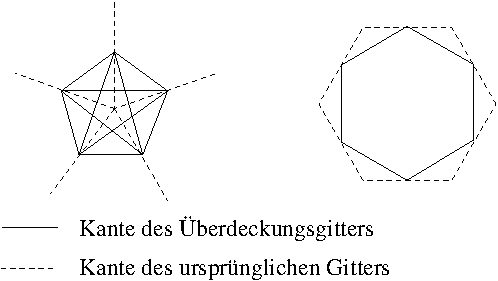
\includegraphics{./Schranken-figs/covering}
  \caption{Links: Der \"Uberdeckungsgraph eines Vertex mit Koordinationszahl $\bar{z}=5$ ist ein dekoriertes $\bar{z}$-Eck. Rechts: In jede Plakette des urspr\"unglichen Gitters wird eine undekorierte Plakette der gleichen Kantenzahl eingeschrieben.}
  \label{fig:covering}
\end{figure}
\\Wir betrachten bond-Perkolation auf einem archimedischen Gitter mit Vertexkonfiguration $(n_1,\ldots,n_{\bar{z}})$ und wollen die Euler-Charakteristik des \"Uberdeckungsgitter bestimmen. Die Euler-Charakteristiken der \"Uberdeckungsgitter werden zweckm\"a"siger\-weise mit der im Kapitel \ref{sec:matchingpoly} beschriebenen Methode f\"ur beliebige dekorierte Mosaike ausgerechnet. Um die Euler-Charakteristik zu bestimmen, m\"ussen wir die erwarteten Anzahlen der unterschiedlichen Vertextypen (siehe Abb. \ref{fig:decoratedcov}) kennen. 
\begin{figure}[htbp]
  \centering
  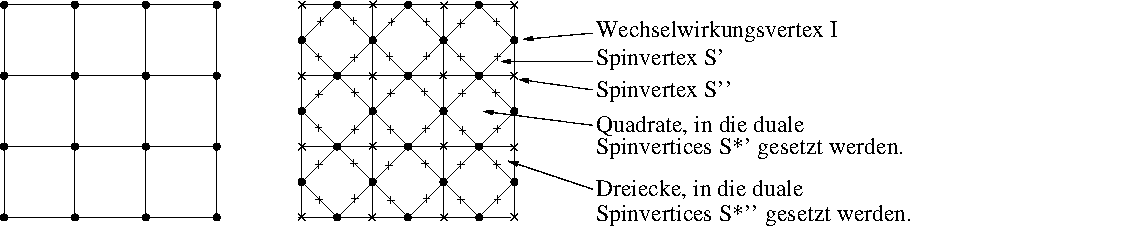
\includegraphics{./Schranken-figs/decratedcov}
  \caption{Links ist ein Ausschnitt des Quadratgitters zu sehen, rechts ist der Wechselwirkungsgraph des \"Uberdeckungsgitters dieses Ausschnitts gezeigt. In alle Plaketten dieses Graphens, werden duale Spinvertices gesetzt.}
  \label{fig:decoratedcov}
\end{figure}
\begin{itemize}
\item Auf jeden Vertex von $G^{cov}$, d.h. auf jede Kante des archimedischen Gitters, wird ein Wechselwirkungsvertex $i\in I$ gesetzt. Diese Vertices sind mit Wahrscheinlichkeit $p$ besetzt.
\item Auf jede Kante des undekorierten Mosaiks von $G^{cov}$ werden Spinvertices $s \in S'$ gesetzt; diese Vertices sind immer vorhanden, werden aber nur gez\"ahlt, wenn mindestens einer der benachbarten Vertices aus $I$ besetzt ist. Das Mosaik hat Koordinationszahl $4$, und der Beitrag der Vertices aus $S'$ pro Wechselwirkungsvertex ist daher $2(1-(1-p)^2)=2(1-q^2)$.
\item In jede dekorierte Plakette von $G^{cov}$ wird ein Spinvertex $s\in S''$ gesetzt und mit allen umgebenden Wechselwirkungsvertices verbunden. Die Kantenzahl dieser Plaketten ist die Koordinationszahl $\bar{z}$ des archimedischen Gitters. Die Zahl dieser Plaketten verh\"alt sich zu der Zahl der Wechselwirkungsvertices wie die Zahl der Vertices zu der Zahl der Kanten des archimedischen Gitters. Wiederum werden Spins $s\in S''$ nur gez\"ahlt, wenn sie nicht isoliert sind. Der Beitrag der Vertices aus $S''$ pro Wechselwirkungsvertex ist daher $\frac{2}{\bar{z}}(1-(1-p)^{\bar{z}})=\frac{2}{\bar{z}}(1-q^{\bar{z}})$. Die Spinmenge $S$ aus Gleichung (\ref{eq:matchingpoly}) ist die Vereinigung aus $S'$ und $S''$.
\item In jede undekorierte Plakette wird ein dualer Spin $s^*\in S^{*'}$ gesetzt. Diese Plaketten entsprechen den Plaketten des archimedischen Gitters. Pro Vertex des archimedischen Gitters gibt es $\frac{1}{n_i}$ Plaketten mit Kantenzahl $n_i$, $i=1,\ldots,\bar{z}$; pro Wechselwirkungsvertex gibt es $\frac{2}{\bar{z}}$ Vertices des archimedischen Gitters und damit $\frac{2}{\bar{z}n_i}$ duale Spins $s^*\in S^{*'}$ pro Wechselwirkungsvertex, wiederum f\"ur $i=1,\ldots,\bar{z}$. Duale Spins werden gez\"ahlt, wenn sie nur von besetzten Wechselwirkungsvertices umgeben sind; Summation \"uber alle $i$ liefert den Beitrag $\sum_{i=1}^{\bar{z}}\frac{2}{\bar{z}n_i}p^{n_i}$.
\item Auch in die Dreiecke, die entstehen, wenn Spins $s\in S''$ mit den umliegenden Vertices aus $I$ verbunden werden, m\"ussen duale Spins $s^*\in S^{*''}$ gesetzt werden. Es gibt $\bar{z}$ dualer Spins $s^*$ pro Spin $s\in S''$ und damit zwei pro Wechselwirkungsvertex. Wenn beide Wechselwirkungsvertices auf den Ecken des Dreiecks besetzt sind, wird der Spin gez\"ahlt, und der Beitrag der dualen Spins aus $S^{*''}$ ist  $2p^2$.
\item Das Mosaik hat Koordinationszahl $4$; dar\"uberhinaus ist jeder Vertex aus $I$ mit zwei Vertices aus $S''$ verbunden und hat daher Koordinationszahl $6$.
\end{itemize}
Mit Gleichung (\ref{eq:matchingpoly}) und den eben bestimmten Gr\"o"sen erh\"alt man f\"ur die mittlere Euler-Charakteristik des \"Uberdeckungsgitter eines archimedischen Gitters mit Vertexkonfiguration $(n_1,\ldots,n_{\bar{z}})$
\begin{equation}
\label{eq:cov}
  \fbox{$\displaystyle \chi_{cov}(p)=p+2(1-q^2)+\frac{2}{\bar{z}}(1-q^{\bar{z}})+2p^2+\sum_{i=1}^{\bar{z}}\frac{2}{\bar{z}n_i}p^{n_i}-6p.$}
\end{equation}
Die Euler-Charakteristiken der \"Uberdeckungsgitter aller archimedischen Gitter, die Nullstellen und Wendepunkte der Euler-Charakteristiken und die bond-Perkolationsschwellen der archimedischen Gitter sind in Tabelle \ref{tab:covering} zusammengetragen. Die Perkolationsschwellen sind von van der Marck \cite{Marck:03} mit Genauigkeit $2*10^{-4}$ bestimmt worden. Um die entsprechenden Werte f\"ur die Laves-Gitter zu erhalten, muss $p$ durch $1-p$ ersetzt werden. Der Plot befindet sich wieder in Abbildung \ref{fig:2dallplots}. F\"ur bond-Perkolationsschwellen gilt, mit Ausnahme des $(3,4,6,4)$-Gitters, $p_0^{(2)}\leq p_c \leq p_0$ falls $p_c \geq \frac{1}{2}$ ist und $p_0^{(2)}\geq p_c \geq p_0$ falls $p_c \leq \frac{1}{2}$ ist.

\begin{table}
\centering
\begin{tabular}{|l|l||r|r|r||r|}
\hline
Vertexkon. & $\frac{\chi_{cov}(p)}{p(1-p)}$& $ p_0^{cov}$&$p_0^{(2)cov}$&$\frac{p_0^{cov}+p_0^{(2)cov}}{2}$&$p_c^{bond}$ \\ \hline
\hline
$3,12^2$ & $1-p-\frac{1}{9}\sum_{i=2}^{10}p^i $& $0.7580$&$0.6863$&$0.7221$&$0.7406(2)$ \\ \hline
$4,6,12$ & $1-p- \frac{2p^2+p^3+p^4}{6}-\frac{1}{18}\sum_{i=5}^{10}p^i $& $0.7054$&$0.6380$&$0.6717$&$0.6935(2)$ \\ \hline
$4,8^2$ & $1-p-\frac{1}{3}p^2-\frac{1}{6}\sum_{i=3}^6p^i $& $0.6964$&$0.6384$&$0.6674$&$0.6768(2)$ \\ \hline
$6^3$ & $1-p-\frac{1}{3}(p^2+p^3+p^4) $& $0.6756$&$0.6231$&$0.6494$&$0.65270\ldots$ \\ \hline
$3,6,3,6$ & $1-2p-\frac{1}{3}(p^2+p^3+p^4) $&$0.5277$&$0.5178$&$0.5228$&$0.5244053(3)$ \\ \hline
$3,4,6,4$ & $1-2p-\frac{1}{6}p^2-\frac{p^3+p^4}{12} $&$0.5134$&$0.5083$&$0.5109$&$0.5250(2)$ \\ \hline
$4^4$& $1-2p$&$0.5$&$0.5$&$0.5$&$0.5$ \\ \hline
$3^4,6$& $1-3p+\frac{1}{15}(23p^2-7p^3-p^4) $&$0.4069$&$0.4332$&$0.4200$&$0.4344(2) $ \\ \hline
$3^2,4,3,4$ & $1-3p+\frac{1}{5}(7p^2-2p^3) $&$0.3992$&$0.4305$&$0.4148$&$0.4142(2) $ \\ \hline
$3^3,4^2$ & $1-3p+\frac{1}{5}(7p^2-2p^3) $&$0.3992$&$0.4305$&$0.4148$&$0.4195(2) $ \\ \hline
$3^6$& $1-4p+\frac{1}{3}(10p^2-5p^3+p^4) $&$0.3244$&$0.3769$&$0.3506$&$0.34729\ldots$ \\ \hline
\end{tabular}
\caption{Euler-Charakteristik und bond-Perkolation auf archimedischen Gittern: Die erste Spalte enth\"alt die Vertexkonfiguration des archimedischen Gitters und die zweite die reduzierte mittlere Euler-Charakteristik des \"Uberdeckungsgitters $\frac{\chi^{cov}(p)}{p(1-p)}$. Bei fast allen Gittern mit bond-Perkolationsschwelle $p_c \geq \frac{1}{2}$ gilt f\"ur die Nullstelle $p_0$ und den Wendepunkt $p_0^{(2)}$ der Euler-Charakteristik $p_0^{(2)}\leq p_c \leq p_0$. F\"ur Gitter mit $p_c<\frac{1}{2}$ gilt $p_0^{(2)}\geq p_c \geq p_0$. Das Mittel aus $p_0$ und $p_0^{(2)}$ liegt nahe bei $p_c$. Die bond-Perkolationsschwellen des Dreiecks- ($3^6$), Sechsecks- ($6^3$) und Quadratgitters ($4^4$) sind exakt bekannt, der Wert f\"ur das Kagom\'egitter ($3,6,3,6$) stammt aus \cite{Suding:99}, alle \"ubrigen aus  \cite{Marck:03}. }
\label{tab:covering}
\end{table}

\begin{figure}[htbp]
  \centering
  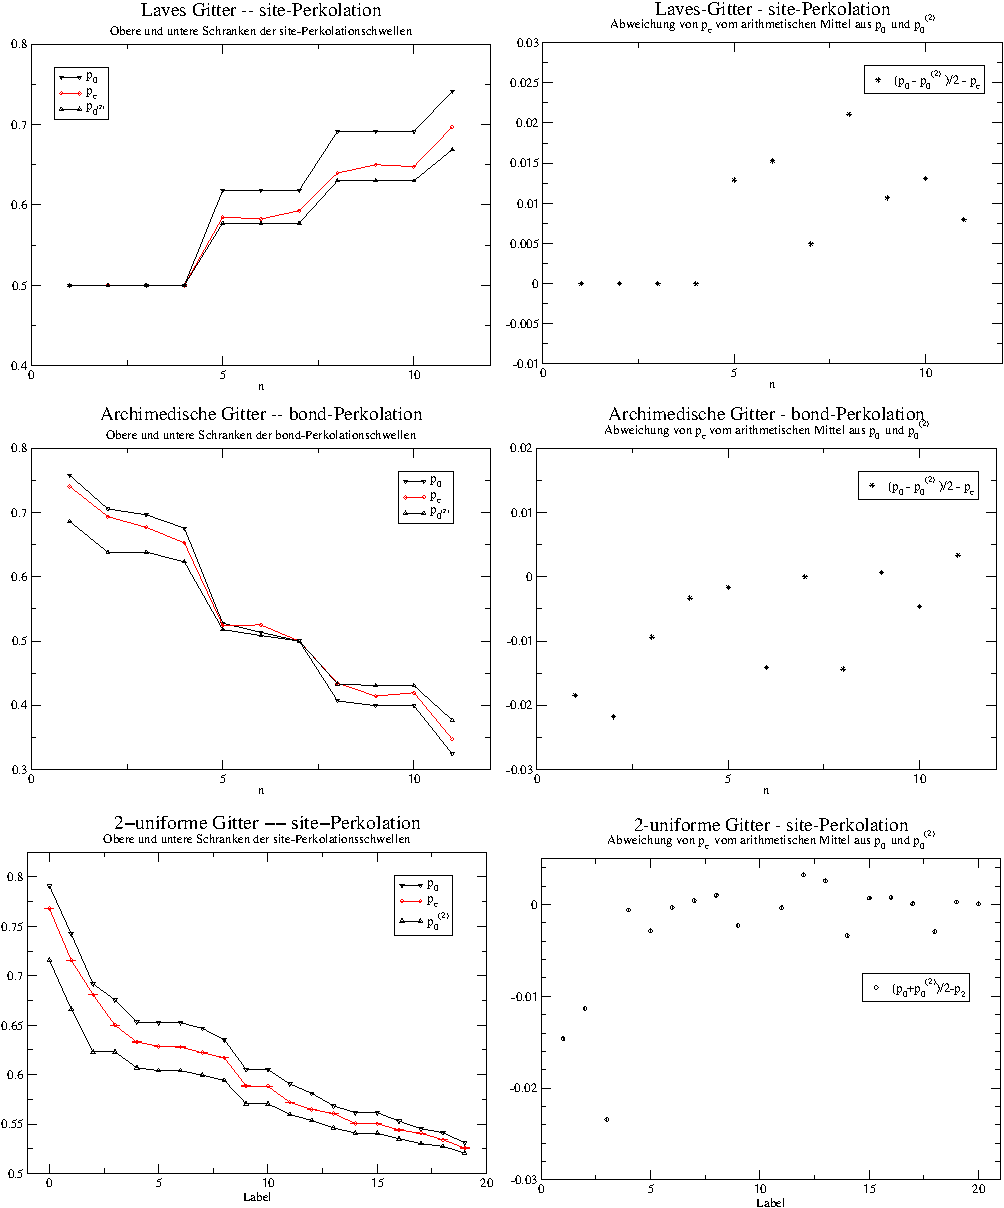
\includegraphics[width=16cm]{./Schranken-figs/2dallplots}
  \caption{In den drei Grafiken auf der linken Seite sind die Nullstellen $p_0$ und Wendepunkte $p_0^{(2)}$ der Euler-Charakteristiken, sowie die Perkolationsschwellen $p_c$ aller regelm\"a"sigen Gitter aufgetragen. In den drei rechten Grafiken ist die Abweichung des arithmetischen Mittels aus $p_0$ und $p_0^{(2)}$ von $p_c$ gezeigt. Die numerischen Werte sind in den Tabellen \ref{tab:covering}, \ref{tab:2-uniform} und \ref{tab:laves} zu finden. Der Plot f\"ur site-Perkolation archimedischer Gitter ist in Abb. \ref{fig:archisite} zu finden.}
  \label{fig:2dallplots}
\end{figure}
\subsection{Irregul\"are Gitter}
Es gibt einige weitere Gitter, deren site-Perkolationsschwellen bekannt sind, die aber nicht in die oben behandelten Kategorien passen. Daher werden sie hier gesondert vorgestellt.\\
Das Bowtie-Gitter hat Vertexkonfiguration $\left[ \frac{1}{2}(4,3,4,3)_1+\frac{1}{2}(4,3^2,4,3^2)_2 \right]$; sein duales Gitter $\left[ \frac{2}{3}(4,6^2)_1+\frac{1}{3}(4,6,4,6)_2 \right]$ (siehe Abb. \ref{fig:bowtie}). F\"ur die Euler-Charakteristiken erh\"alt man mit Gleichung (\ref{eq:2-uniform})
\begin{eqnarray}
  \chi(p) & = &p(1-p)\left(1-\frac{3}{2}p-\frac{1}{2}p^2 \right)\\
 \chi^{dual}(p)& = & p(1-p)\left(1-\frac{2p+2p^2+p^3+p^4}{3} \right).
\end{eqnarray}
\begin{figure}[bp]
  \centering
  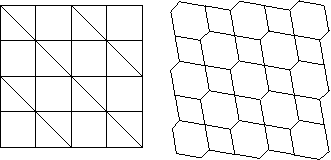
\includegraphics{./Schranken-figs/bowtie}
  \caption{Bowtie- (links) und duales Bowtie-Gitter}
  \label{fig:bowtie}
\end{figure}
\\Das Penrose-Gitter ist ein nichtperiodisches Gitter, dessen Plaketten alle Vierecke sind \cite{Gruenbaum:86}. Seine mittlere Euler-Charakteristik ist daher die gleiche wie beim Quadratgitter.\\
Auch f\"ur die zuf\"alligen Delauny- und Voronoi-Gitter \cite{Weygaert:91} l\"asst sich in zwei Dimensionen die mittlere Euler-Charakteristik bestimmen. Das Delauny-Gitter besteht nur aus Dreiecken und die Euler-Charakteristik ist $\chi^{delauny}(p)=p(1-p)(1-2p)$. Die Euler-Charakteristik des Voronoi-Gitters h\"angt von der Verteilung $s_n$ der Plaketten mit Kantenzahl $n$ ab, die aber nur approximativ bekannt ist. Der Mittelwert der Kantenzahl ist $6$ und die Koordinationszahl fast sicher $z=3$. Damit erh\"alt man 
\begin{equation}
\label{eq:voronoi}
  \chi^{Voronoi}(p)=p-1+\frac{3}{2}(1-p^2)-\frac{1}{2}\sum_{n\geq 3}s_n(1-p^n).
\end{equation}
Das \"Uberdeckungsgitter des Voronoi-Gitters entspricht einem Kagom\'e-Gitter, in dem die Sechsecke durch unregelm\"a"sige Polygone ersetzt sind. Die Kantenzahl der unregelm\"a"sigen Polygone hat die Verteilung $s_n$, und die Euler-Charakteristik ist mit Gl. (\ref{eq:cov}) 
\begin{equation}
\label{eq:voronoibond}
  \chi^{Vor.cov.}(p) =  p+2(1-q^2)+\frac{2}{3}(1-q^3)-6p+2p^2+\frac{2}{3}\sum_{n\geq 3}s_np^n.
\end{equation}
Die Werte der Perkolationsschwellen $p_c$ der Gitter, sowie der Nullstellen $p_0$ und Wendepunkte $p_0^{(2)}$ der Euler-Charakteristiken sind in Tabelle \ref{tab:irreg} zusammengetragen. In allen F\"allen gilt $p_0\geq p_c \geq p_0^{(2)}$. Steven van der Marck \cite{Marck:03} hat noch f\"ur eine Reihe weiterer Gitter Perkolationsschwellen bestimmt. Viele dieser Gitter enthalten aber Substrukturen und zeigen die Grenzen der G\"ultigkeit der Faustregel auf. Auf diese Gitter wird im n\"achsten Kapitel genauer eingegangen.\\
\begin{table}
\centering
\begin{tabular}{|l|r|r|r||r|}
\hline
Name &  $ p_0$&$p_0^{(2)}$&$\frac{p_0+p_0^{(2)}}{2}$&$p_c$ \\ \hline
\hline
bowtie & $0.5616$ &$0.5408$&$0.5512$&$0.5474(8)$\cite{Marck:97} \\ \hline
bowtie dual & $0.7048$&$0.6411$&$0.6730$&$0.6653(6)$\cite{Marck:97} \\ \hline
Penrose &  $0.6180$&$0.5774$&$0.5977$&$0.5837(2)$\cite{Yonezawa:88} \\ \hline
Delauny & $1/2$ & $1/2$ & $1/2$&$1/2$ \\ \hline
Voronoi &$0.7548$&$0.6787$&$0.7167$&-- \\ \hline
Voronoi bond  & $0.6855$&$0.6288$&$0.6572$&$0.6670(1)$\cite{Hsu:99}  \\ \hline
\end{tabular}
\caption{Perkolation und Euler-Charakteristik unregelm\"a"siger Gitter: F\"ur die Nullstellen $p_0$ und die Wendepunkte $p_0^{(2)}$ der Euler-Charakteristiken und die Perkolationsschwellen $p_c$ gilt $p_0^{(2)}\leq p_c\leq p_0$. Das Mittel aus $p_0$ und $p_0^{(2)}$ ist nahe bei $p_c$. Abgesehen von der Zeile ``Voronoi bond'', beziehen sich alle Werte auf site-Perkolation. Um $p_0$ und $p_0^{(2)}$ des Voronoi-Gitters zu erhalten, wurde eine approximative Verteilung $s_n$ der Plaketten mit Kantenzahl $n$ aus \cite{Stoyan:96} verwendet.}
\label{tab:irreg}
\end{table}


\subsection{Zuf\"allig dekorierte Mosaike}
\label{sec:decorated}
Ein Gitter heisst dekoriertes Mosaik, wenn es aus einem planaren Gitter (Mosaik) besteht, dessen Plaketten teilweise um allen diagonalen Kanten erweitert wurden. Die Vertices auf dem Rand einer solchen Plakette sind dann alle durch Kanten verbunden, und die Plakette heisst dekoriert (siehe Kapitel \ref{sec:dualitaet}). Um zu untersuchen, wie sich $p_c$ mit dem Bruchteil der dekorierten Plaketten eines Mosaiks \"andert, kann man Gitterplaketten mit Wahrscheinlichkeit $m$ dekorieren, und $p_c$ f\"ur eine Reihe verschiedener Werte von $m$ bestimmen. Die mittlere Euler-Charakteristik dieser statistisch dekorierten Mosaike kann mit Gl. (\ref{eq:matchingpoly}) bestimmt werden. Dazu m\"ussen die Kardinalit\"aten der Vertexmengen und die mittlere Koordinationszahl des Wechselwirkungsgraphs (siehe Abb. \ref{fig:randomdec}) bestimmt werden. 
\begin{figure}[bp]
  \centering
  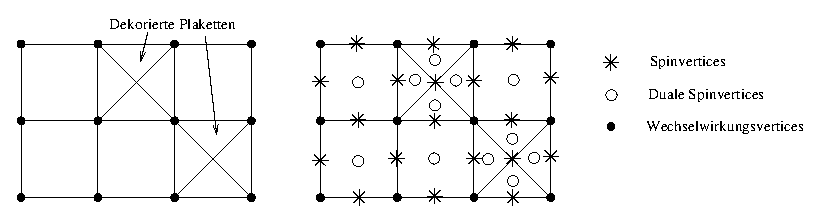
\includegraphics{./Schranken-figs/randomdec}
  \caption{Teil eines dekorierten Quadratgitters (links) und der resultierende Wechselwirkungsgraph (rechts).}
  \label{fig:randomdec}
\end{figure}
\begin{itemize}
\item Wechselwirkungsvertices sitzen auf jedem Gitterplatz und sind mit Wahrscheinlichkeit $p$ besetzt.
\item Spinvertices $s\in S$ sitzen auf allen Kanten und in dem mit Wahrscheinlichkeit $m$ dekorierten Plaketten. Wenn das Mosaik nur Plaketten mit Kantenzahl $n$ und Vertices mit Koordinationszahl $z$ hat, gibt es pro Wechselwirkungsvertices im Mittel $\frac{z}{2}(1-(1-p)^2)+m\frac{z}{n}(1-(1-p)^n)$ Spins. Bei einem komplizierteren Gitter treten mehr Terme auf, die aber analog berechnet werden k\"onnen.
\item Duale Spinvertices $s^*\in S^*$ werden in alle undekorierten Plaketten und in die Dreiecke, in die die dekorierten Plaketten durch den Wechselwirkungsgraph zerschnitten werden, gesetzt. Sie werden nur dann gez\"ahlt, wenn alle umliegenden Wechselwirkungsvertices besetzt sind. Haben alle Plaketten Kantenzahl $n$, gibt es pro Wechselwirkungsvertex $(1-m)\frac{z}{n}p^n+mzp^2$ duale Spins.
\item Die Koordinationszahl eines Wechselwirkungsvertex ist die des Mosaiks $z$, zuz\"uglich der Zahl der ihn umgebenden dekorierten Plaketten. Die mittlere Koordinationszahl ist $\bar{z}=z+\sum_{i=1}^z im^i(1-m)^{z-i}{ i \choose z }$.
\end{itemize}    
Mit Gleichung (\ref{eq:matchingpoly}) und den oben bestimmten Gr\"o"sen l\"asst sich die Euler-Charakteristik ausrechen.
\\Die Perkolationsschwellen komplement\"ar dekorierter Mosaike erg\"anzen sich zu 1. F\"ur $m=1/2$ sind die zuf\"allig dekorierten Mosaike im statistischen Sinn selfmatching, und $p_c$ sowie $p_0$ sind $1/2$. Perkolation auf zuf\"allig dekorierten Gittern ist eine Form der gemischten Perkolation. Vertices werden mit Wahrscheinlichkeit $p$ und Plaketten mit Wahrscheinlichkeit $m$ besetzt. Kanten sind immer besetzt.\\
Ich habe f\"ur das Quadrat-, Sechseck- und Kagom\'e-Gitter, sowie das $3^3,4^2$- und das $3,12^2$-Gitter die Perkolationsschwelle in Abh\"angigkeit von $m$ berechnet. Details der Simulation sind im Anhang \"uber numerische Methoden zusammengefasst. Die Perkolationsschwelle f\"allt vom leeren zum vollst\"andig dekorierten Mosaik ab (siehe Abb. \ref{fig:dekoratedpc}). Die Perkolationsschwellen von Gittern mit einem Anteil an dekorierten Plaketten von $m\in[0,1]$ und $1-m$ erg\"anzen sich zu $1\pm 0.01$, wie aufgrund der statistischen matching-Eigenschaft zu erwarten war. Die Genauigkeit der Simulation ist nicht sehr hoch, da f\"ur jedes Gitter 100 verschiedene Werte von $m$ simuliert werden mussten. Die Fehlerabsch\"atzungen ergeben sich einfach aus den Fluktuationen von $p_c(m)$ um eine glatte Kurve.
\begin{figure}[htbp]
  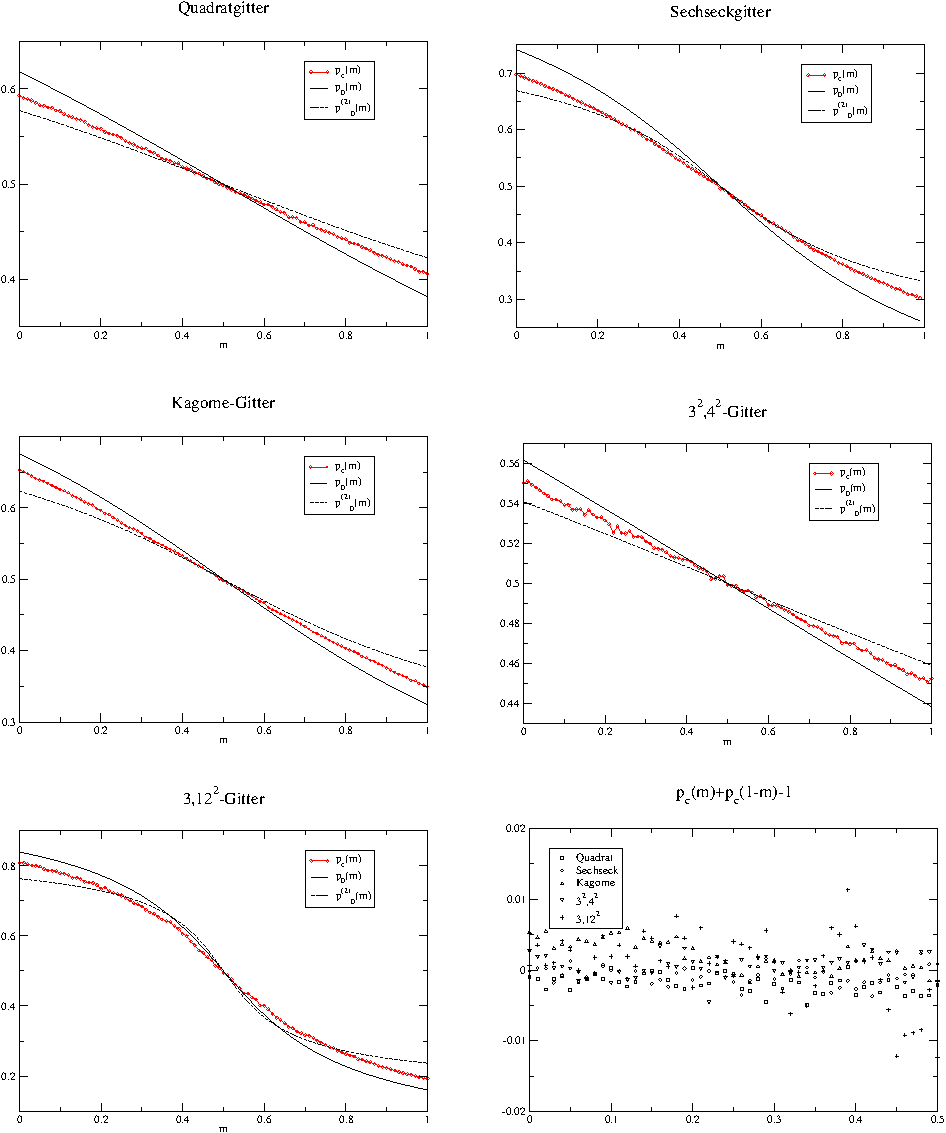
\includegraphics{./Schranken-figs/matching}
  \caption{Die Grafiken zeigen die Perkolationsschwelle $p_c(m)$ in Abh\"angigkeit vom Bruchteil $m$ der dekorierten Plaketten f\"ur die f\"unf untersuchten Gitter. Zus\"atzlich sind Nullstelle $p_0(m)$ und Wendepunkt $p_0^{(2)}(m)$ der Euler-Charakteristik eingezeichnet. Rechts unten ist die Abweichung von $p_c(m)+p_c(1-m)$ von $1$ f\"ur alle Gitter aufgetragen.}
\label{fig:dekoratedpc}
\end{figure}
\begin{figure}[htbp]
  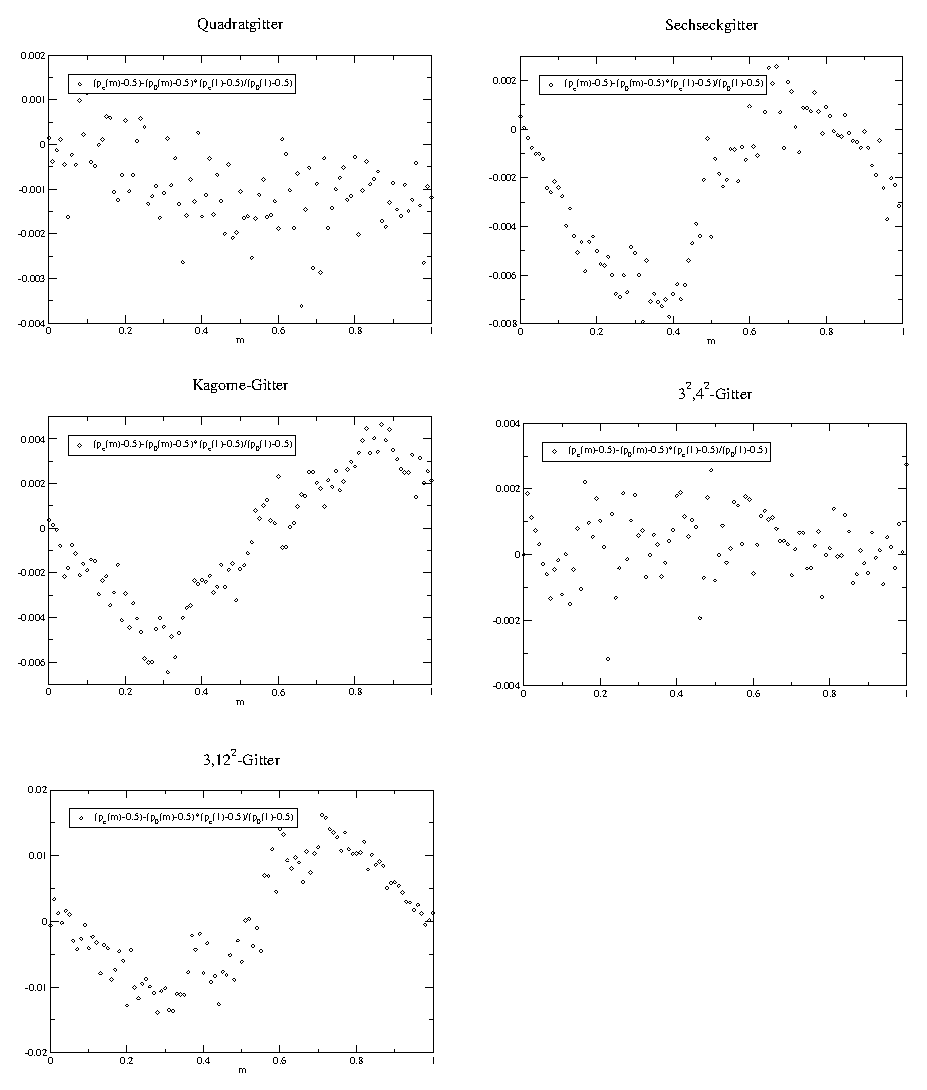
\includegraphics{./Schranken-figs/scale}
  \caption{Die Perkolationsschwelle $p_c(m)$ von Gittern, deren Plaketten mit Wahrscheinlichkeit $m$ dekoriert sind, ist fast identisch mit der reskalierten Nullstelle der Euler-Charakteristik $(p_0(m)-0.5)\frac{p_c(1)-0.5}{p_0(1)-0.5}+0.5$. F\"ur die f\"unf untersuchten Gitter ist die Differenz beider Gr\"o"sen aufgetragen.}
\label{fig:scale}
\end{figure}
\\W\"ahrend f\"ur Gitter mit Perkolationsschwellen nahe $\frac{1}{2}$ die Kurve $p_c(m)$ kaum von einer Geraden abweicht, ist beim Sechseck- und $3,12^2$-Gitter ein geschwungener Verlauf deutlich erkennbar (siehe Abb. \ref{fig:dekoratedpc}). F\"ur alle Gitter und alle $m$ ist die Nullstelle der Euler-Charakteristik im Rahmen der Genauigkeit der Simulation f\"ur $p_c<\frac{1}{2}$ eine untere und f\"ur $p_c>\frac{1}{2}$ eine obere Schranke. F\"ur den Wendepunkt der Euler-Charakteristik gilt das komplement\"are Verhalten, anders als f\"ur $m=0$ und $m=1$, nicht. Die Kurve $p_0(m)$ hat sehr \"ahnliche Form wie $p_c(m)$, und beide Kurven k\"onnen durch Skalierung fast zur Deckung gebracht werden. In Abbildung \ref{fig:scale} ist die Differenz von $p_c(m)$ und $(p_0(m)-0.5)\frac{p_c(1)-0.5}{p_0(1)-0.5}+0.5$ f\"ur die untersuchten Gitter dargestellt. Die Abweichung liegt innerhalb der Fehlergrenzen der Simulation, zeigt aber f\"ur Gitter mit gro"sem $p_c$ systematische Variation.\\
Die Daten stimmen innerhalb der Fehlergrenzen mit bekannten Perkolationsschwellen f\"ur undekorierte oder vollst\"andig dekorierte Gitter \"uberein \cite{Suding:99}.


\section{Euler-Charakteristik gro"ser Cluster}
\label{sec:scaling}
Bei allen bisher untersuchten zweidimensionalen Gitter, mit Ausnahme der bond-Perkolation auf dem $(3,4,6,4)$-Gitter, ist $p_0$ gr\"o"ser als $p_c$, wenn $p_c>\frac{1}{2}$, und kleiner, wenn $p_c<\frac{1}{2}$ ist. Auch die Untersuchungen an zuf\"allig dekorierten Gitter haben die Vermutung sehr gut best\"atigt, dass $p_0>p_c$ ist, falls $p_c>\frac{1}{2}$ ist, und, dass $p_0<p_c$ ist, falls $p_c<\frac{1}{2}$ ist. Zusammen mit den archimedischen Gittern ist die vermutete Beziehung zwischen $p_0$ und $p_c$ also auf einer gro"sen Zahl von Gittern, wenn auch nur numerisch, verifiziert worden. Im Folgenden soll der Versuch gemacht werden, die Ursache dieses Sachverhalts zu verstehen.\\

An der Perkolationsschwelle divergiert die Korrelationsl\"ange und es gibt, abgesehen von der Gitterkonstanten, keine charakteristische L\"angenskala. Die Skalenannahme sagt voraus, dass die Clusterkonfiguration auf jeder Skala, die gro"s gegen den Gitterabstand ist, qualitativ gleich aussieht. Stauffer \cite{Stauffer:95} hat f\"ur die Zahl der Cluster pro Vertex $n_s$ der Gr\"o"se $s$ in der N\"ahe von $p_c$ ($\Delta p=p-p_c$)
\begin{equation}
  \label{eq:skalenann}
   n_s=q_0 s^{-\tau}f(\Delta pq_1s^{\sigma})
\end{equation}
als Skalenrelation vorgeschlagen. Die Parameter $q_0,q_1$ und $p_c$ h\"angen vom betrachteten Gitter ab; die \"ubrigen Gr\"o"sen und die Funktion $f(z)$ sind universell.\\
Seien nun $q_0,q_1$ und $p_c$ die nicht-universellen Parameter des betrachteten Gitters und $q_0^*,q_1^*$ und $1-p_c$ die des matching Gitters. Die Summen
\begin{equation}
  \sum_{s=s_0}^{\infty}n_s(p) \qquad \text{und} \qquad \sum_{s=s_0}^{\infty}n_s^*(q)
\end{equation}
sind die Zahlen der Cluster bzw. L\"ocher, die gr\"o"ser als ein gewisses $s_0$ sind. Ihre Differenz ist die Euler-Charakteristik pro Vertex, zu der nur Cluster der Gr\"o"se $s\geq s_0$ beitragen. Mit der Skalenannahme ergibt sich
\begin{equation}
   \chi_{s_0}(p):=\sum_{s=s_0}^{\infty}n_s(p)-n_s^*(1-p)=\sum_{s=s_0}^{\infty}s^{-\tau}\left[ q_0f(\Delta pq_1s^{\sigma})-q_0^*f(-\Delta pq_1^*s^{\sigma})\right].
\end{equation}
Die Wahrscheinlichkeiten, dass ein Vertex in einem Cluster oder einem Loch der Gr\"o"se $s\geq s_0$ ist, sind durch 
\begin{equation}
  \sum_{s=s_0}^{\infty}sn_s(p)+P_{\infty}(p) \qquad \text{und} \qquad \sum_{s=s_0}^{\infty}sn_s^*(q)+P_{\infty}^*(q)
\end{equation}
gegeben.
F\"ur die Differenz beider Gr\"o"sen gilt mit der Skalenannahme
\begin{equation}
\begin{split}
   [p-q]_{s_0}& :=\sum_{s=s_0}^{\infty}s\left[n_s(p)-n_s^*(1-p)\right]+P_{\infty}(p)-P_{\infty}^*(q) \\ & =\sum_{s=s_0}^{\infty}s^{-\tau+1}\left[ q_0f(\Delta pq_1s^{\sigma})-q_0^*f(-\Delta pq_1^*s^{\sigma})\right]+P_{\infty}(p)-P_{\infty}^*(q).
\end{split}
\end{equation}
Bei $p=p_c$ vereinfachen sich die Beziehungen zu 
\begin{equation}
   \chi_{s_0}(p_c)=(q_0-q_0^*)f(0)\sum_{s={s_0}}^{\infty}s^{-\tau}
\end{equation}
und 
\begin{equation}
   [p_c-q_c]_{s_0}=(q_0-q_0^*)f(0)\sum_{s=s_0}^{\infty}s^{-\tau+1}.
\end{equation}
Die Summen lassen sich durch Integrale n\"ahern und man erh\"alt
\begin{equation}
   \chi_{s_0}(p_c)=(q_0-q_0^*)f(0)\frac{s_0^{-\tau+1}}{\tau-1}
\end{equation}
und
\begin{equation}
   [p_c-q_c]_{s_0}=(q_0-q_0^*)f(0)\frac{s_0^{-\tau+2}}{\tau-2}.
\end{equation}
Der Exponent $\tau$ hat in zwei Dimensionen vermutlich den Wert $\frac{187}{91}$, ist also gr\"o\ss er als $2$. Daher haben $\chi_{s_0}(p_c)$ und $[p_c-q_c]_{s_0}$ das gleiche Vorzeichen und ihr Verh\"altnis ist
\begin{equation}
   \fbox{$\displaystyle \frac{\chi_{s_0}(p_c)}{[p_c-q_c]_{s_0}}=\frac{\tau-2}{\tau-1}s_0^{-1}=\frac{5}{96s_0}.$}
\end{equation}
Wenn sich das Skalenverhalten bis zu kleinen Clustern qualitativ fortsetzt, ist $\chi(p_c)$ positiv und das Verh\"altnis $\frac{\chi(p_c)}{p_c-q_c}$ sollte ungef\"ahr $\frac{5}{96}$ betragen. F\"ur archimedische Gitter gilt dies im Rahmen der Erwartungen (siehe Tabelle \ref{tab:archiscale}).
\begin{table}
\centering
\begin{tabular}{|l|r|r|}
\hline
Gitter &$\frac{\chi(p_c)}{p_c-q_c}$ ($s_0=1$) &$\frac{\chi(p_c)}{p_c-q_c}-\frac{5}{96}$ \\
\hline
$3,12^2$ & $ 0.0284$&$-0.0237$\\
$4,6,12$ & $ 0.0381$&$-0.0140$\\
$4,8^2$ &$0.0478$&$-0.0043$\\
Sechseckg.&$0.0649$&$0.0128$ \\
Kagom\'eg. &$0.0387$&$-0.0134$\\
$3,4,6,4$&$ 0.0534$&$0.0014$ \\
Quadratg. &$0.0727$&$0.0207$\\
$3^3,6$ &$0.0361$&$-0.0160$\\
$3^2,4,3,4$ &$ 0.0538$&$0.0017$\\
$3^3,4^2$ &$0.0574$ &$0.0054$\\
Dreiecksg. &-- &--\\\hline
\end{tabular}
\caption{Euler-Charakteristik archimedischer Gitter bei $p=p_c$.}
\label{tab:archiscale}
\end{table}
\\F\"ur das Quadratgitter sind die Clusterzahlen sowohl f\"ur n\"achste, als auch f\"ur \"ubern\"achste Nachbarschaften bis $s=12$ bekannt \cite{Mertens:90}, und $\chi_{s_0}(p_c)$ sowie $[p_c-q_c]_{s_0}$ k\"onnen durch Abziehen der bekannten Beitr\"age der Cluster $s<s_0$ von $\chi(p_c)$ und $[p_c-q_c]=2p_c-1$ berechnet werden. Schon f\"ur $s_0\geq 3$ lassen sich die so gewonnen Werte gut an ein Potenzgesetz fitten (siehe Abb. \ref{fig:analytisch_pc_fig}). Die Werte der Fitparameter stimmen aber nur m\"a"sig mit den Erwartungen \"uberein.
\begin{figure}[tbp]
  \centering
  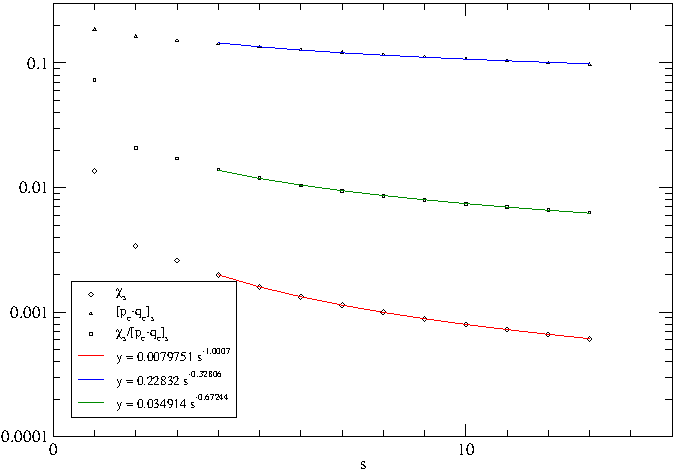
\includegraphics{./Schranken-figs/analytisch_pc_fig}
  \caption{Euler-Charakteristik $\chi_s(p_c)$ und $[p_c-q_c]_s$ (siehe Text) auf dem Quadratgitter f\"ur $s=1,\ldots,13$. Die Kurven sind Fitkurven an die Werte $s\geq3$. Zur Vereinfachung der Darstellung hat der Plot eine logarithmische Ordinate.}
  \label{fig:analytisch_pc_fig}
\end{figure}
\\Da die Clusterzahlen f\"ur gro"ser Cluster nicht exakt bekannt sind, m\"ussen Resultate f\"ur gr\"o"sere $s_0$ aus Monte-Carlo-Simulationen gewonnen werden. Hierzu wird mit dem im Appendix \ref{sec:numerik} vorgestellten Programm eine Perkolationskonfiguration erzeugt und die Clusterverteilung (siehe Abschnitt \ref{sec:numerikverteilung}) ausgewertet. Die Simulationen wurden f\"ur site-Perkolation auf dem Quadrat- und Sechseckgitter sowie f\"ur bond-Perkolation auf dem Sechseckgitter durchgef\"uhrt. Die Kantenl\"ange der simulierten Gitter betrug $L=2048$. Die Ergebnisse sind in sehr guter \"Ubereinstimmung mit dem erwarteten Skalenverhalten. Auch die numerischen Werte f\"ur die Exponenten und das Verh\"altnis $\frac{\chi_{s_0}(p_c)}{[p_c-q_c]_{s_0}}$ stimmen sehr gut mit den Vorhersagen der Skalenannahme \"uberein. Die gewonnen Daten und die ermittelten Fitparameter sind in Abb. \ref{fig:scalinglimit} dargestellt.\\
\begin{figure}[htbp]
  \centering
  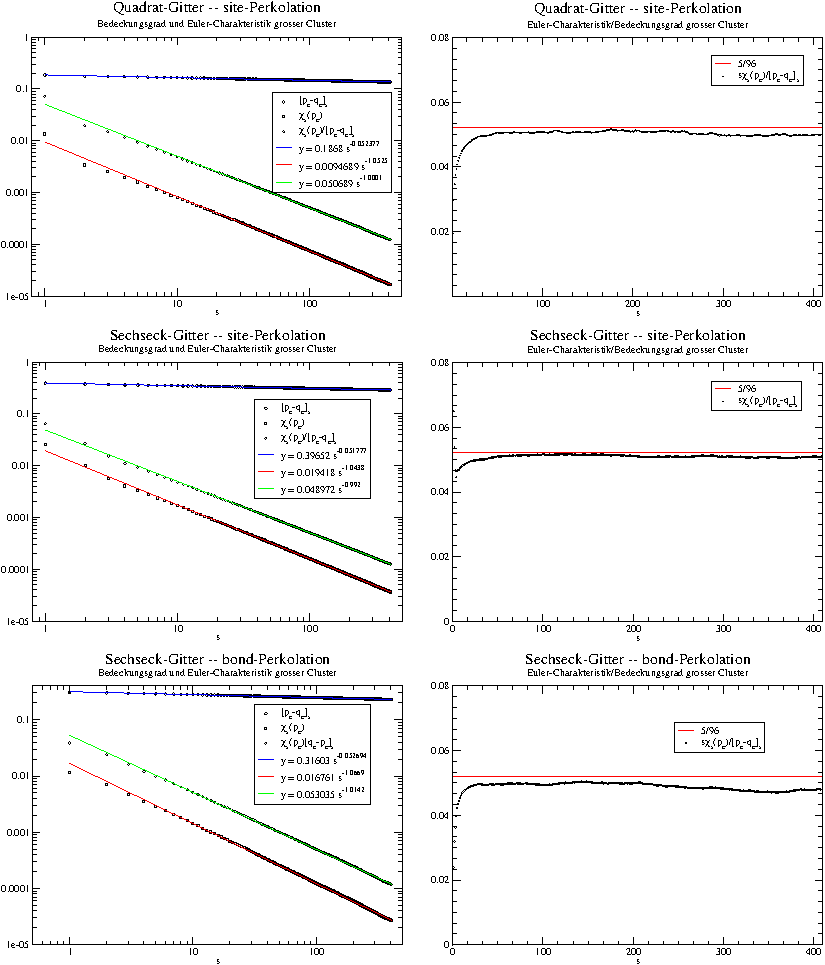
\includegraphics{./Schranken-figs/scalinglimit}
  \caption{Simulationsergebnisse f\"ur die Clusterverteilung bei $p_c$ der site-Perkolation auf dem Quadrat- und Sechseckgitter, sowie bond-Perkolation auf dem Sechseckgitter. Auf der linken Seite sind $\chi_s$, $\chi_s/[p_c-q_c]_s$ und $[p_c-q_c]_s$ doppelt-logarithmisch aufgetragen. Rechts  ist $s\chi_s/[p_c-q_c]_s$ und das erwartete Skalenverhalten $5/96$ dargestellt.}
  \label{fig:scalinglimit}
\end{figure}

Mit der Skalenannahme aus Gleichung (\ref{eq:skalenann}) kann auch die Nullstelle von $n_s(p)-n_s^*(1-p)$ f\"ur gro"se $s$ durch die nicht-universellen Parameter der Gitter ausgedr\"uckt werden. 
\begin{equation}
      n_s(p)-n_s^*(1-p)=q_0 s^{-\tau}f((p-p_c)q_1s^{\sigma})-q_0^* s^{-\tau}f((p_c-p)q_1^*s^{\sigma}).
\end{equation}
F\"ur die Nullstelle von $n_s(p)-n_s^*(1-p)$ ergibt sich die Bedingung ($\Delta p=p_0-p_c$)
\begin{equation}
      q_0 s^{-\tau}f(\Delta p q_1s^{\sigma})=q_0^* s^{-\tau}f(-\Delta p q_1^*s^{\sigma}).
\end{equation}
Angenommen $f(z)$ l\"asst sich um $z=0$ entwickeln, erh\"alt man
\begin{equation}
\begin{split}
 & q_0(f(0)+f'(0)\Delta p q_1s^{\sigma}+\frac{1}{2}f''(0)(\Delta p q_1s^{\sigma})^2+\ldots) \\ & =  q_0^* (f(0)-f'(0)\Delta p q_1^*s^{\sigma}+\frac{1}{2}f''(0)(\Delta p q_1^*s^{\sigma})^2+\ldots).
\end{split}
\end{equation}
Nach Potenzen in $\Delta p s^\sigma$ geordnet ergibt sich
\begin{equation}
  f(0)(q_0-q_0^*)+f'(0)(q_0q_1+q_0^*q_1^*)\Delta p s^\sigma+\frac{1}{2}f''(0)(q_0q_1^2-q_0^*{q_1^{*}}^2)(\Delta ps^{\sigma})^2+\ldots=0.
\end{equation}
$\Delta p s^\sigma$ muss f\"ur alle $s$ L\"osung des Polynoms mit konstanten Koeffizienten sein. F\"ur die L\"osung gilt $\Delta p s^\sigma=const.$ oder $\Delta p=const.* s^{-\sigma}$. Falls $\Delta ps^\sigma \ll 1$, kann man Terme h\"oherer Ordnung vernachl\"assigen. Eine konsistente Skalenfunktion $f(x)$ hat ihr einziges Maximum bei negativem $x$ \cite{Stauffer:95}, und daher ist $f'(0)<0$. $\Delta p$ hat dann das gleiche Vorzeichen wie $q_0-q_0^*$ und ist mit obigen Argumenten f\"ur $p_c>1/2$ positiv. Die bekannten Clusterzahlen f\"ur das Quadratgitter best\"atigen das Skalenverhalten, und ein Fit an die Werte $s=6,\ldots,12$ liefert einen Exponenten $\sigma=0.38$. Es wird vermutet, dass $\sigma$ den Wert $\frac{36}{91}\approx 0.396$ hat. \\ 

Mit der Skalenhypothese l\"asst sich die Beobachtung, dass f\"ur $p_c>\frac{1}{2}$ die Nullstelle der Euler-Charakteristik \"uber $p_c$ liegt, begr\"unden. Allerdings liefern kleine Cluster mit Abstand den gr\"o"sten Beitrag zur Euler-Charakteristik und gerade f\"ur diese ist die Skalenannahme nicht g\"ultig. Wenn sich das Skalenverhalten qualitativ auf kleine Cluster fortsetzt, sollte aber $p_c<p_0$ gelten, wenn $p_c>\frac{1}{2}$ ist.  

\section{Euler-Charakteristiken in drei Dimensionen}
Um den Zusammenhang zwischen $p_0$ und $p_c$ in drei Dimensionen weiter zu untersuchen, wurde die mittlere Euler-Charakteristik verschiedener dreidimensionaler Gitter berechnet, deren Perkolationsschwellen bekannt sind. Wie schon im Kapitel \ref{sec:chimittel} diskutiert, m\"ussen zur Berechnung der Euler-Charakteristik von Clustern auf dreidimensionalen Gittern, Zellen um die Vertices gefunden werden, die die Nachbarschaftsverh\"altnisse des Gitters widerspiegeln. Die Wahl solcher Zellen ist in der Regel nicht eindeutig. Bei Gittern, deren Wigner-Seitz-Zellen (WSZ) geeignet sind, um die Euler-Charakteristik zu berechnen, sind die WSZ als nat\"urliche Zellen vorgegeben. Dennoch kann man auch durch Wahl anderer Zellen Zusammenhangsverh\"altnisse erzeugen, die denen des Gitters entsprechen. Die Zahl der Zellen, mit denen eine Zelle einen nichtleeren Durchschnitt hat, ist bei diesen Zellen aber i. A. eine andere als bei den WSZ, und man erh\"alt unterschiedliche Euler-Charakteristiken. 
\\Sind geeignete Zellen gefunden, werden sie wie immer mit Wahrscheinlichkeit $q=1-p$ besetzt. Wir berechnen die mittlere Euler-Charakteristik dieser Figuren $\bar{\chi}(1-p)$. In drei Dimensionen gilt f\"ur die Euler-Charakteristik des geeignet abgeschlossenen Komplements $\chi(p)=\bar{\chi}(1-p)$. Wir werden uns auf Ergebnisse und wesentliche Aspekte beschr\"anken und technische Details der Rechnungen und Konstruktionen in den Appendix verbannen.

\subsection{Gitterstapel}
Die einfachste M\"oglichkeit dreidimensionale Gitter zu erhalten, ist, Ebenen zweidimensionaler Gitter \"ubereinander zu legen, und jeden Vertex mit den Vertices \"uber und unter ihm zu verbinden. Solche Gitter hei"sen Gitterstapel.\\
Prismen mit den dualen Plaketten der zweidimensionalen Gitter als Grundfl\"ache sind geeignete Zellen, um die Euler-Charakteristik auszurechnen. Die H\"ohe der Prismen ist der Gitterebenenabstand, und die Gittervertices sollen im Schwerpunkt der Prismen liegen. Diese Prismen haben nur mit den Prismen der n\"achsten Nachbarn im zweidimensionalen Gitter und mit denen der senkrecht \"uber und unter ihnen liegenden Gittervertices eine Fl\"ache gemein. Sie sind daher geeignet $\chi(p)$ zu berechnen. \\
Durch die Gitterebenen ist eine Schichtstruktur vorgegeben und die Euler-Charakteristik wird zweckm\"a"sigerweise mit der Schnittrekursion ausgerechnet. Die Schnittebenen stehen senkrecht auf Symmetrieachse der Prismen. Das Schnittmuster besteht aus besetzten und unbesetzten dualen Plaketten des zweidimensionalen Gitters. Die mittlere Euler-Charakteristik dieser Muster ist die des vollst\"andig dekorierten zweidimensionalen Gitters $\bar{\chi}_{2}(q)$. Die Schnittmuster \"andern sich nur, wenn die Schnittebene von einer Prismenschicht in die n\"achste wandert. Dort, wo sich zwei Prismenschichten ber\"uhren, sind die Plaketten des Schnittmusters mit Wahrscheinlichkeit $1-(1-q)^2$ besetzt. Jeder andere Schnitt entspricht dem zweidimensionalen Gitter mit Besetzungswahrscheinlichkeit $q$. Die Differenz der Euler-Charakteristiken beider Schnitte ist $\bar{\chi}(q)$:
\begin{equation}
  \bar{\chi}(q)=\bar{\chi}_{2}(1-(1-q)^2)-\bar{\chi}_{2}(q).
\end{equation}
In zwei Dimensionen gilt $\chi_2(p)=-\bar{\chi}_2(1-p)$ und daher
\begin{equation}
  \bar{\chi}(q)=-\chi_{2}((1-q)^2)+\chi_{2}(1-q)
\end{equation}
Weiterhin gilt in drei Dimensionen $\chi(p)=\bar{\chi}(1-p)$ und f\"ur die Euler-Charakteristik des Gitterstapels gilt
\begin{equation}
  \chi(p)=-\chi_{2}(p^2)+\chi_{2}(p).
\end{equation} \\
Die Nullstellen der Euler-Charakteristiken der Gitterstapel aller archimedischer Gitter und Laves-Gitter, sowie des Bowtie- und des dualen Bowtie-Gitters sind zusammen mit den bekannten site-Perkolationsschwellen in Tabelle \ref{tab:stacked} angegeben. Die Nullstellen $p_0$ sind bei allen Gittern gr\"o"ser als $p_c$. Die Ergebnisse sind in Abbildung \ref{fig:3dallplots} grafisch dargestellt. 
\begin{table}
  \centering
  \begin{tabular} {|r|r|r||r|r|}
\hline
Nr. & $p_0$ & $p_c$\cite{Marck:97} & $p_0^{dual}$ &$ p_c^{dual}$\cite{Marck:97} \\ \hline
1 &$0.50934$&--&$0.32878$&--\\ \hline
2 &$0.47709$&--&$0.32878$&--\\ \hline
3 &$0.47504$&$0.3840(4)$&$0.32878$&$0.2524(4)$ \\ \hline
4 &$0.46434$&$0.3701(4)$&$0.32878$&$0.2623(4)$ \\ \hline
5 &$0.42098 $&$0.3346(4)$&$0.39401$&$0.2998(4)$ \\ \hline
6 &$0.40698$&--& $0.39401$&--\\ \hline
7 &$0.39401 $&$0.3114(4)$&$0.39401$&$0.3114(4)$ \\ \hline
8 &$0.37384$&--& $0.43546$&--\\ \hline
9 &$0.36184$&--&  $0.43546$&--\\ \hline
10 &$0.36184 $&$0.2872(4)$& $0.43546$&$0.3394(4)$ \\ \hline
11 &$0.32878 $&$0.2623(4)$&$0.46435$&$0.3701(4)$ \\ \hline
bowtie &$0.36184$&$ 0.2822(4)$ &$0.44098$ &$0.3480(4)$ \\ \hline
\end{tabular}
\caption{Euler-Charakteristik und site-Perkolation auf Gitterstapeln: Die erste Spalte enth\"alt die Nummer (1-11) des zweidimensionalen archimedischen Gitters oder ``bowtie'' f\"ur das Bowtie-Gitter. In der zweiten und dritten Spalte sind die Nullstellen $p_0$ der Euler-Charakteristik und, falls bekannt, die Perkolationsschwellen $p_c$ der Gitterstapel der zweidimensionalen Gitter angegeben. In der vierten und f\"unften Spalte sind $p_0$ und $p_c$ der Stapel der dualen Gitter angegeben. }
\label{tab:stacked}
\end{table}

\subsection{Einfach-kubisches Gitter}
Das einfach-kubische Gitter (sc-Gitter) ist als Gitterstapel des Quadratgitters schon behandelt worden, und seine Euler-Charakteristik als Beispiel in Kapitel \ref{sec:chimittel} berechnet worden. Hier soll die Euler-Charakteristik f\"ur den Fall, dass Vertices des Gitters verbunden sind, wenn ihre dualen W\"urfel (WSZ) an Fl\"achen oder an Kanten zusammenh\"angen, berechnet werden. Details der Rechnung befinden sich im Anhang \ref{sec:appsc}. Ein Gittervertex hat 18 Nachbarn. Ein W\"urfel um einen Vertex hat mit den W\"urfeln von 26 anderen Vertices einen nichtleeren Durchschnitt. Die Euler-Charakteristik ist
 \begin{equation}
  \chi_{18-26}^{sc}(p)=p(1-p)(p^6+p^5+p^4+p^3+4p^2-8p+1).
\end{equation}

 
\subsection{fcc-Gitter}
\label{sec:schrfcc}
Das fcc-Gitter (face centered cubic) ist ein einfach-kubisches Gitter (sc-Gitter), bei dem in die Fl\"achen der W\"urfel zus\"atzliche Vertices gesetzt werden (siehe Abb. \ref{fig:fcc}). Alternativ kann man das Gitter auch als vier jeweils um die halbe L\"ange der drei Fl\"achendiagonalen gegeneinander verschobene sc-Gitter auffassen. Dann liegt ein Vertex mittig in je einer Fl\"ache der anderen drei sc-Gitter und hat damit zw\"olf je eine halbe Fl\"achendiagonale entfernte Nachbarn. Die Wigner-Seitz-Zelle (WSZ) des fcc-Gitters ist ein rhombisches Dodekaeder. WSZ entstehen durch den Schnitt von Ebenen mittig und senkrecht auf den Gitterverbindungen. Jede Fl\"ache der WSZ entspricht einer Gitterkante, und die WSZ sind zur Berechnung der Euler-Charakteristik geeignet.
\begin{figure}[htbp]
  \centering
  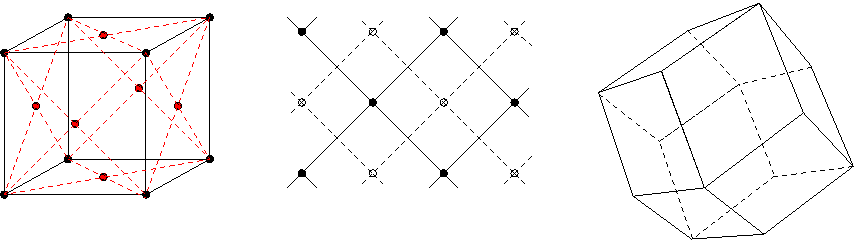
\includegraphics{./Schranken-figs/fcc}
  \caption{Links ein W\"urfel mit Vertices in allen Fl\"achen. In der Mitte sind die beiden durch Projektion entlang einer W\"urfelkante entstehenden Quadratgitter dargestellt. Rechts ist eine Skizze der WSZ des fcc-Gitters, ein rhombisches Dodekaeder, zu sehen.}
  \label{fig:fcc}
\end{figure}
Die Anzahlen der Zellen verschiedener Dimensionen lassen sich leicht bestimmen (siehe Appendix \ref{sec:appfcc}), und man erh\"alt f\"ur die Euler-Charakteristik
\begin{equation}
  \chi^{fcc-WSZ}_{12-18}(p)=p(1-p)(1-5p+3p^2+p^3+p^4).
\end{equation}
Neben den zw\"olf Zellen, die die WSZ an Fl\"achen ber\"uhrt, gibt es sechs weitere WSZ, die sie nur an einer Ecke ber\"uhrt. Somit gibt es insgesamt $18$ Zellen, mit denen eine WSZ einen nichtleeren Durchschnitt hat.\\
Alternativ zu den WSZ k\"onnen auch Prismen quadratischer Grundfl\"ache als Zellen benutzt werden. Das fcc-Gitter ist n\"amlich ein Stapel gegeneinander verschobener Quadratgitter (siehe Abb. \ref{fig:fcc}). Prismen mit quadratischer Grundfl\"ache sind Zellen, die die Zusammenhangsverh\"altnisse des Gitters widerspiegeln, denn sie haben mit den Zellen innerhalb der Ebene je eine Fl\"ache gemein, und obere und untere Fl\"achen \"uberlappen mit den Fu"s- bzw. Kopffl\"achen von vier Prismen aus den darunter bzw. dar\"uber liegenden Ebenen. An den senkrechten Kanten sto"sen die Prismen innerhalb einer Ebene mit den \"ubern\"achsten Nachbarn auf dem Quadratgitter zusammen. Eine Zelle kann also mit 16 Nachbarzellen einen nichtleeren Durchschnitt haben, statt 18 bei der WSZ. Die Euler-Charakteristik, die man mit den Prismen erh\"alt (siehe Appendix \ref{sec:appfcc}), ist
\begin{equation}
  \chi^{fcc-Qu}_{12-16}(p)=p(1-p)(1-5p+3p^2+2p^3).
\end{equation}
Zum Vergleich der beiden Euler-Charakteristiken sind sie links in Abbildung \ref{fig:fcc+bccplot} aufgetragen. Bis zur ersten Nullstelle, die in beiden F\"allen zw\"olf Nachbarn entspricht, unterscheiden sie sich kaum. F\"ur $p>0.3$ ist der Unterschied deutlich erkennbar.
\begin{figure}[htbp]
  \centering
  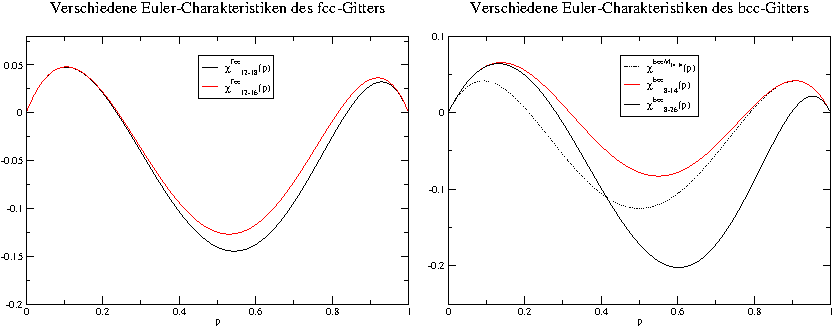
\includegraphics{./Schranken-figs/chiplot}
  \caption{Verschiedene Euler-Charakteristiken des fcc- (links) und bcc-Gitters (rechts).}
  \label{fig:fcc+bccplot}
\end{figure}

\subsection{bcc-Gitter}
Das bcc-Gitter (body centered cubic) entsteht, wenn in die Mitte jedes W\"urfels des sc-Gitter ein weiterer Vertex gesetzt wird (siehe Abb. \ref{fig:bcc}). Man erh\"alt das bcc-Gitter auch durch zwei \"uberlagerte, um eine halbe Raumdiagonale gegeneinander verschobene, sc-Gitter. Die n\"achsten Nachbarn eines Vertex des bcc-Gitter sind die acht Vertices auf den Ecken des umgebenden W\"urfels. Die WSZ des bcc-Gitters hat 14 Fl\"achen, davon acht Sechsecke, die den Gitterkanten entsprechen, und sechs Quadrate, die den Kanten der sc-Untergitter entsprechen. 
F\"ugt man die Kanten der sc-Gitter zum bcc-Gitter hinzu, erh\"alt man ein Gitter mit 14 Nachbarn. An jeder Kante der WSZ sto"sen nur drei und an jeder Ecke nur vier Zellen zusammen. D.h. es sto"sen keine Zellen zusammen, die nicht ohnehin eine gemeinsame Fl\"ache haben, und das Komplement hat die gleichen Zusammenhangsverh\"altnisse. Das bcc-Gitter mit 14 Nachbarn ist in dieser Hinsicht das dreidimensionale Analogon des zweidimensionalen Dreiecksgitters. Das 14er bcc-Gitter wurde in \cite{Likos:95} behandelt; die Euler-Charakteristik ist
\begin{equation}
  \chi_{14-14}^{bcc}(p)=p(1-p)(1-6p+6p^2).
\end{equation}
\begin{figure}[tbp]
  \centering
  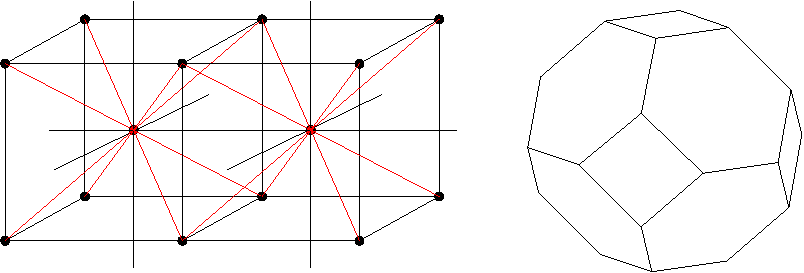
\includegraphics{./Schranken-figs/bcc}
  \caption{Bcc-Gitter: Links ist ein Ausschnitt des bcc-Gitter zu sehen. Die Gitterkanten sind mit roten Linien eingezeichnet; Kanten der sc-Untergitter sind schwarz gezeichnet. Rechts ist die Wigner-Seitz-Zelle (WSZ) des bcc-Gitter gezeigt.}
  \label{fig:bcc}
\end{figure}Um eine Euler-Charakteristik zu erhalten, die die Zusammenhangsverh\"altnisse des bcc-Gitter mit acht Nachbarn widerspiegelt, kann man entweder eine komplizierte Zelle (siehe Abbildung \ref{fig:bcc_nonconvex_app} und Kapitel \ref{sec:appbcc}) w\"ahlen, oder zwei WSZ nur dann als benachbart betrachten, wenn sie sich an einem Sechseck ber\"uhren. Zwei WSZ, die sich an einem Quadrat ber\"uhren, gelten dann nur als benachbart, wenn sie einen gemeinsamen besetzten Gitternachbarn haben (siehe Kapitel \ref{sec:mixedbcc}). Die Euler-Charakteristiken, die man mit den unterschiedlichen Methoden erh\"alt, unterscheiden sich im Wesentlichen in der Zahl der Zellen, mit denen ein abgeschlossene Zelle einen nichtleeren Durchschnitt hat. W\"ahrend eine nichtkonvexe Zelle mit 26 anderen Zellen einen nichtleeren Durchschnitt hat, sind es bei der WSZ nur 14. 
\begin{eqnarray}
  \chi_{8-26}^{bcc}(p)&=&p(1-p)(1-3p-3p^2+3p^3+3p^4)\\
  \chi_{8-14}^{bcc}(p)&=&p(1-p)(1-3p-3p^2+9p^3-3p^4).
\end{eqnarray}
Um die drei unterschiedlichen Euler-Charakteristiken zu vergleichen, sind im rechten Teil der Abb. \ref{fig:fcc+bccplot} aufgetragen. Wenn die Nachbarschaftszahlen $z$ bzw. $\bar{z}$ zweier Euler-Charak\-ter\-istiken \"ubereinstimmen, unterschieden sie f\"ur kleine bzw. gro"se $p$ kaum. So f\"allt $\chi_{8-26}^{bcc}(p)$ mit $\chi_{8-14}^{bcc}(p)$ f\"ur $p<0.3$ fast zusammen, w\"ahrend sie f\"ur gro"se $p$ stark unterschiedlich sind. F\"ur $p>0.7$ sind dagegen $\chi_{8-14}^{bcc}(p)$ und $\chi_{14-14}^{bcc}(p)$ sehr \"ahnlich. Im Bereich $p\approx \frac{1}{2}$ unterscheiden sich alle sehr stark, da die Bedingungen, unter denen ein ``Tunnel'' entstehen kann, unterschiedlich sind.

\subsection{Diamantgitter}
Das Diamantgitter ist ein fcc-Gitter mit zweiatomiger Basis, also kein Bravaisgitter. Wenn ein Vertex auf einem fcc-Vertex liegt, liegt der andere bei $(\frac{1}{4},\frac{1}{4},\frac{1}{4})$ auf der W\"urfeldiagonale des sc-Teilgitters. Ein Vertex hat vier n\"achste Nachbarn, die auf den Ecken eines Tetraeders um den Vertex liegen.
 
\subsubsection{Nichtkonvexe Zelle mit 4er-Nachbarschaft}
Um der Topologie des Diamantgitters mit seinen vier n\"achsten Nachbarn Rechnung zu tragen, ist eine Zelle n\"otig, die nur die Zellen der vier n\"achsten Nachbarn an einer Fl\"ache ber\"uhrt. Wie diese Zellen aussehen, und wie die Euler-Charakteristik berechnet wird, ist im Anhang \ref{sec:appdiamantnonconvex} beschreiben. Man erh\"alt f\"ur die Euler-Charakteristik 
\begin{equation}                     
        \chi^{Diamant}_{4-47}(p)=p(1-p)\left(\frac{p^{12}+p^{11}+p^{10}+p^9+p^8+p^7+p^6+p^5}{2}-p^4-p^3-p^2-p+1 \right).
\end{equation}
Diese Zellen ber\"uhren insgesamt 47 Zellen an Ecken, Kanten oder Fl\"achen.

\subsubsection{Konvexe Zellen mit 4er-Nachbarschaft}
Nun betrachten wir eine WSZ des fcc-Gitters und halbieren sie senkrecht zur Basisachse (siehe Abb. \ref{fig:fcc_half}). Die gemeinsame Schnittfl\"ache und die drei Rhomben auf der gegen\"uberliegenden Seite geh\"oren zu einer Gitterkante des Diamantgitters. Alle anderen Seiten entsprechen keinen Gitternachbarschaften, und zwei Zellen sollen \"uber diese Seiten nur zusammenh\"angen, wenn sie einen gemeinsamen n\"achsten Nachbarn haben. Analog zur Prozedur aus Kapitel \ref{sec:mixedbcc} kann so eine Euler-Charakteristik des Diamantgitters berechnet werden. Die im Anhang \ref{sec:appdiamantconvex} beschriebene Rechnung liefert: 
\begin{equation}
  \chi^{Diamant}_{4-19}(p)=p(1-p)(p^8+p^7+p^6+p^5-4p^4+2p^3-p^2-p+1).
\end{equation}
Eine halbierte WSZ kann mit 19 anderen Zellen einen nichtleeren Durchschnitt haben. \\

In Abbildung \ref{fig:diamantplot} sind die beiden Euler-Charakteristiken des Diamantgitters aufgetragen. Beide Euler-Charakteristiken sind f\"ur kleine $p$ \"ahnlich. Dadurch, dass die Zellen zur Berechnung von $\chi^{Diamant}_{4-47}(q)$ sehr viele andere Zellen an Ecken oder Kanten ber\"uhren, entstehen Tunnel sehr viel einfacher als bei Verwendung der konvexen Zellen, und $\chi^{Diamant}_{4-47}(p)$ ist f\"ur $p\approx0.5$ kleiner als $\chi^{Diamant}_{4-19}(p)$.
\begin{figure}[tbp]
  \centering
  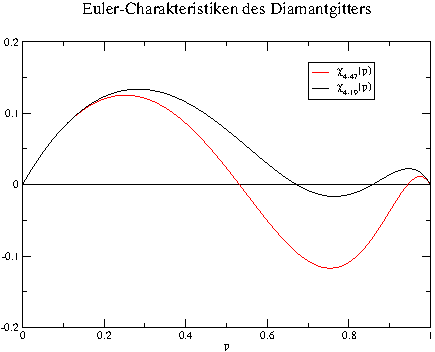
\includegraphics{./Schranken-figs/chidiamant}
  \caption{Verschiedene Euler-Charakteristiken des Diamantgitters.  }
  \label{fig:diamantplot}
\end{figure}

\section{Euler-Charakteristik und Perkolation in drei Dimensionen}
Jeder Euler-Charakteristik der dreidimensionalen Gitter  haben wir ein Paar von Zahlen $(z,\bar{z})$ zugeordnet. Die erste Zahl $z$ ist die Koordinationszahl des Gitters. Die zweite Zahl $\bar{z}$ ist die Zahl der Zellen, mit denen eine abgeschlossene Zelle einen nichtleeren Durchschnitt haben kann. Wenn man auf dem Gitter alle Vertices verbindet, deren Zellen einen nichtleeren Durchschnitt haben, erh\"alt man ein Gitter mit der Topologie der unbesetzten Bereiche. Dieses Gitter hat die Koordinationszahl $\bar{z}$. Die Gitter mit Zusammenhangsverh\"altnissen der unbesetzten Bereiche entsprechen den matching-Gittern in zwei Dimensionen. Da die Wahl der Zellen aber nicht eindeutig ist, sind auch die ``matching''-Gitter in drei Dimensionen nicht eindeutig. 
\\Jede der berechneten Euler-Charakteristiken dreidimensionaler Gitter hat zwei Nullstellen zwischen null und eins. Die kleinere von beiden markiert den \"Ubergang von isolierten Clustern zu vernetzten Strukturen, in denen Tunnel \"uberwiegen. Sie wird der Perkolationsschwelle des Gitter mit $z$ Nachbarn zugeordnet.  Die zweite Nullstelle markiert den \"Ubergang vernetzter Strukturen zu isolierten Einschl\"ussen und wird daher der Perkolationsschwelle der unbesetzten Bereiche zugeordnet. Wenn explizit die Euler-Charakteristik $\bar{\chi}(q)$ der unbesetzten Vertices, d.h. des ``matching''-Gitters, betrachtet wird, sind die Rollen von $z$ und $\bar{z}$ vertauscht und $\bar{\chi}_{\bar{z},z}(q)=\chi_{z,\bar{z}}(p)$. 
\\Auch in drei Dimensionen best\"atigt sich die Vermutung, dass die Nullstelle der Euler-Charakteristik in der Regel eine obere Schranke an die Perkolationsschwelle ist. Das gilt sowohl f\"ur die Perkolation auf den untersuchten Gittern, als auch f\"ur die Perkolation auf den ``matching''-Gittern, sofern deren Perkolationsschwellen bekannt sind. Nur die Euler-Charakteristik des sc-Gitters mit 18 Nachbarn f\"allt aus der Reihe, was wohl daran liegt, dass sowohl das Gitter selbst, als auch das ``matching''-Gitter sehr hohe Koordinationszahlen haben. In Abbildung \ref{fig:3dallplots} sind die Perkolationsschwellen $p_c$ und die Nullstellen $p_0$ der Euler-Charakteristik f\"ur alle behandelten Gitter aufgetragen. Die numerischen Werte der Nullstellen und Perkolationsschwellen sind in den Tabellen \ref{tab:stacked} und \ref{tab:3dall} zusammengefasst. Tr\"agt man die Nullstellen der Euler-Charakteristiken gegen $z$ auf (Plot in Abb. \ref{fig:pooverz}), beobachtet man in etwa $p_0\sim \frac{1}{z}$.


 
\begin{table}
  \centering
  \begin{tabular} {|l|r|r|r||r|}
\hline
Name & $z$&$\bar{z}$ & $p_0$ & $p_c$ \\ \hline
Diamant (nicht konvex)&$4$&$47$&$0.5318$ & $0.4286(4)$ \\ \hline
Diamant (konvex)&$4$&$19$&$0.6722$ & $0.4286(4)$ \\ \hline
sc (WSZ)&$6$&$26$&$0.3940$&$0.3114(4)$\\ \hline
bcc (nicht konvex)& $8$&$26$ &$0.2825$&$0.2458(4)$ \\ \hline
bcc (konvex)&$8$&$14$&$0.3185$&$0.2458(4)$ \\ \hline
fcc (WSZ)&$12$&$18$&$0.2370$&$0.1994(2)$ \\ \hline
fcc (Prisma)&$12$&$16$&$0.2401$& $0.1994(2)$\\ \hline
bcc (WSZ)&$14$&$14$&$0.2113$ &$0.175$\\ \hline 
sc (WSZ)&$18$&$26$&$0.1344$ & $0.137$\\ \hline \hline
bcc (WSZ)&$14$&$8$&$0.2185$&$0.175$ \\ \hline 
fcc (Prisma)&$16$&$12$&$0.1851$& -- \\ \hline
fcc (WSZ)&$18$&$12$&$0.1616$&  $0.136$\\ \hline
Diamant (konvex)&$19$&$4$&$0.1425$ & -- \\ \hline
sc (WSZ)&$26$&$6$&$0.1139$& $0.097$\\ \hline
bcc (nicht konvex)&$26$&$8$&$0.1033$&$0.095$\\ \hline
Diamant (nicht konvex)& $47$&$4$&$0.0561$ & --  \\\hline  

\end{tabular}
\caption{Dreidimensionale Gitter: Nullstellen $p_0$ der verschiedenen Euler-Charakteristiken im Vergleich zu den Perkolationsschwellen $p_c$. Die zur Berechnung der Euler-Charakteristik verwendeten Zellen und die resultierenden Koordinationszahlen besetzter und unbesetzter Zellen sind jeweils angegeben. Eintr\"age unterhalb des Doppelstrichs geh\"oren zu ``matching''-Gittern. Vierstellige Perkolationsschwellen mit Fehlergrenzen stammen aus \cite{Marck:97}, die \"ubrigen aus \cite{Essam:72}. Letztere sind vermutlich sehr ungenau. }
\label{tab:3dall}
\end{table}

\begin{figure}[htbp]
  \centering
  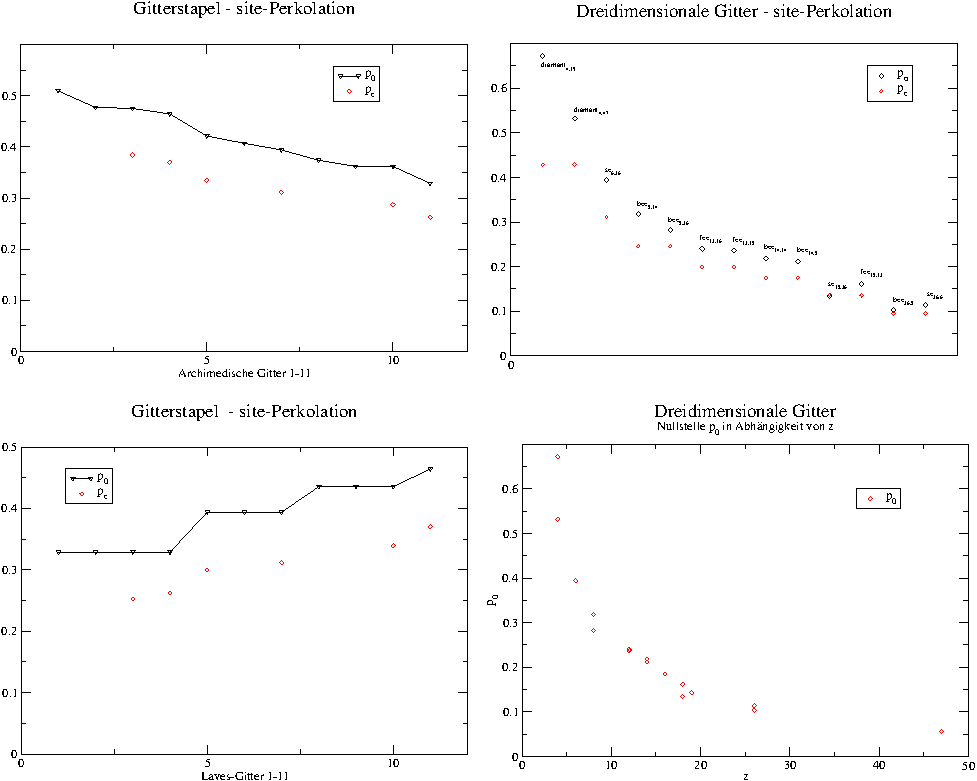
\includegraphics[height=22cm]{./Schranken-figs/3d}
  \caption{Ergebnisse in drei Dimensionen: Die oberen beiden Grafiken zeigen die Nullstellen $p_0$ der Euler-Charakteristik und Perkolationsschwellen $p_c$ f\"ur die Gitterstapel der archimedischen Gitter (oben) und der Laves-Gitter (Mitte). Der unterste Plot enth\"alt $p_0$ und $p_c$ der \"ubrigen untersuchten Gitter.}
  \label{fig:3dallplots}
\end{figure}
\begin{figure}[htbp]
  \centering
  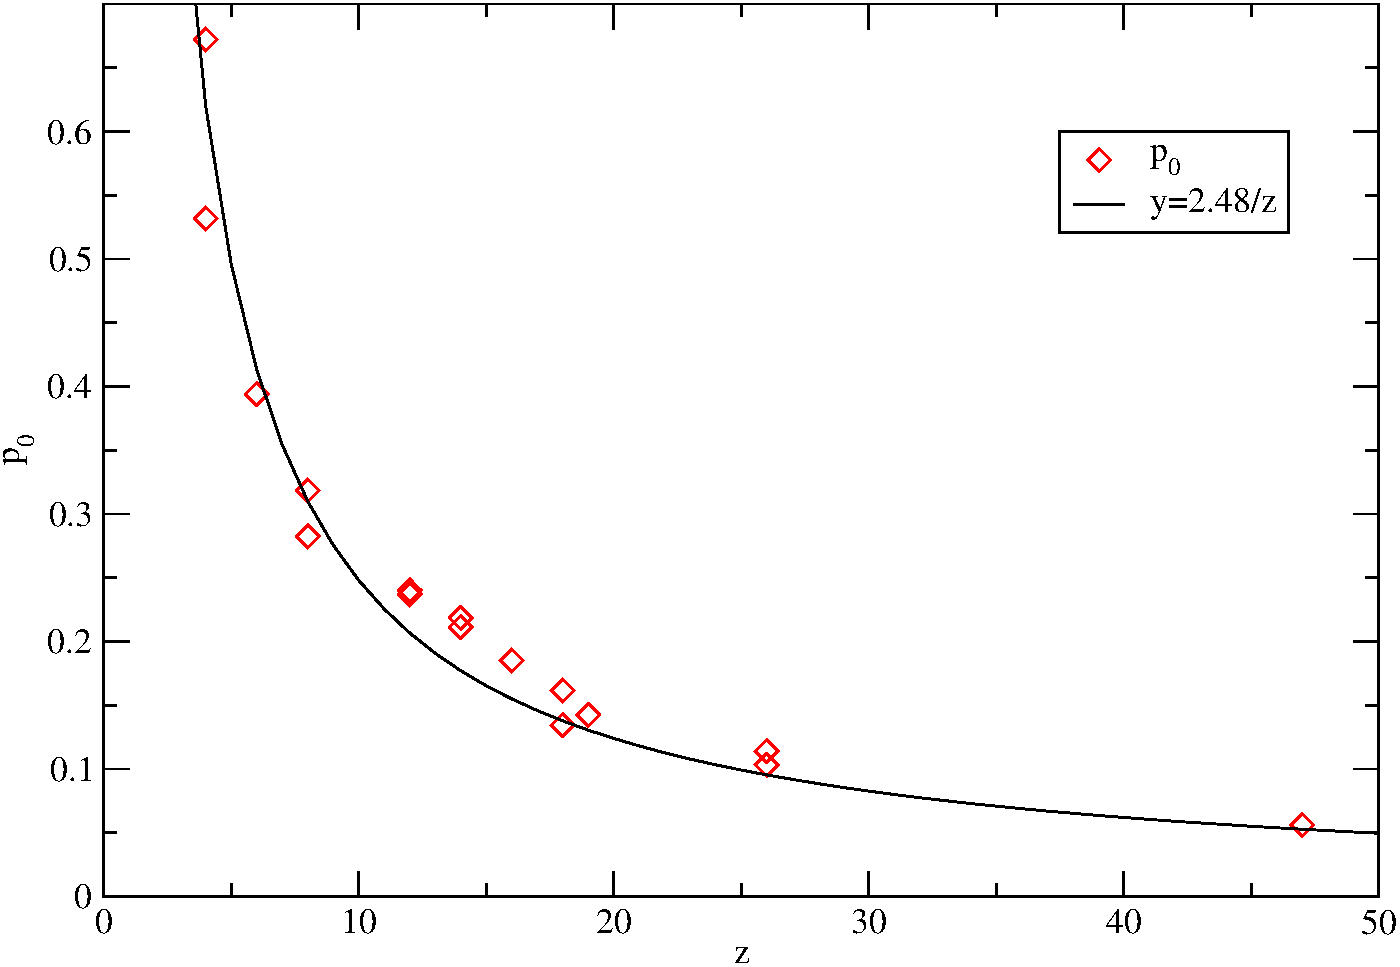
\includegraphics[height=6cm]{./Schranken-figs/pooverz_fig}
  \caption{Variation der Nullstelle $p_0$ der Euler-Charakteristik mit der Zahl der Nachbarn $z$ eines Vertex. Es gilt in etwa $p_0\sim 1/z$. Siehe auch Tabelle \ref{tab:3dall}. }
 \label{fig:pooverz}
\end{figure}

\section{Bond-site-Perkolation}
In Kapitel \ref{sec:mixed} wurde eine Methode vorgestellt, mit der die mittlere Euler-Charakteristik von Konfigurationen, wie sie bei bond-site-Perkolation entstehen, berechnet werden kann. Hier wird die Nullstelle der so berechneten Euler-Charakteristiken mit den bond-site-Perkolationsschwellen der Gitter verglichen.
\\Der kritische Ort eines gemischten bond-site-Perkolationsproblem mit Besetzungswahrscheinlichkeiten $p_s$ und $p_b$ f\"ur Vertices und Kanten ist eine Kurve $[p_s^*(t),p_b^*(t)]_c$ in der $(p_s,p_b)$-Ebene mit einem geeigneten Parameter $t$. Die Kurve l\"asst sich in der Regel sowohl durch $p_b^*$ als auch durch $p_s^*$ parametrisieren. In Ref. \cite{Yanuka:90} wird folgende empirische Beziehung f\"ur die bond-site-Perkolationsschwellen $[p_s^*(t),p_b^*(t)]$ vorgestellt:
\begin{equation}
\label{eq:bondsitepc}
  \frac{\ln p^*_s}{\ln p^*_b}+\frac{\ln p_c^{site}}{\ln p_c^{bond}}=1.
\end{equation}
Die Parameter $p_c^{site}$ und $p_c^{bond}$ sind die Perkolationsschwellen der reinen site- bzw. bond-Perkolation. Die durch Gl. \ref{eq:bondsitepc} gegebene Kurve stimmt bis auf wenige Promille mit den Simulationsergebnissen f\"ur bond-site-Perkolation \"uberein. Die G\"ultigkeit von Gl. \ref{eq:bondsitepc} wurde in Ref. \cite{Tarasevich:99} weiter untersucht, und es wurde sehr gute \"Ubereinstimmung f\"ur zweidimensionale Gitter und Abweichungen von maximal einem Prozent f\"ur h\"oher dimensionale Gitter festgestellt. Die Gl. \ref{eq:bondsitepc} l\"asst sich nach $p^*_b$ oder $p^*_s$ aufl\"osen und man erh\"alt f\"ur die kritische site-Besetzungswahrscheinlichkeit $p^*_s$ bei gegebenem $p_b^*\in [p_c^{bond},1]$
\begin{equation}
\label{eq:bondsitefit}
p^*_s\left(p^*_b\right)=p_c^{site}\left[p^*_b\right]^{-\frac{\ln p_c^{site}}{\ln p_c^{bond}}}.
\end{equation}
Die Genauigkeit dieser empirischen Formel reicht f\"ur den Vergleich mit der Nullstelle der Euler-Charakteristik aus, und statt Simulationsdaten wird f\"ur $[p^*_s,p^*_b]$ die Gleichung \ref{eq:bondsitefit} benutzt.\\
Die mittlere Euler-Charakteristik pro Vertex $\chi(p_s,p_b)$ ist ein Polynom in $p_s$ und $p_b$. $\chi(p_s,p_b)$ hat einige allgemeine Eigenschaften: Ist $p_b=0$, so besteht die Anordnung aus isolierten, abgeschlossenen Zellen und $\chi(p_s,0)=p_s$. F\"ur $p_s=0$ sind \"uberhaupt keine Zellen vorhanden und $\chi(0,p_b)=0$. Der Fall $p_b=1$ entspricht der \"ublichen site-Perkolation und $\chi(p_s,1)=\chi^{site}(p_s)$. Der letzte Extremfall mit $p_s=1$ entspricht einer speziellen Geometrie der bond-Perkolation, bei der, ausgehend von isolierten Zellen, nach und nach Verbindungen durch Verschmelzen von $(d-1)$-Nachbarschaften hinzugef\"ugt werden. $\chi(1,p_b)$ unterscheidet sich von der Euler-Charakteristik, die durch \"Ubergang zum \"Uberdeckungsgitter erhalten wurde.
\begin{figure}[tbp]
  \centering
  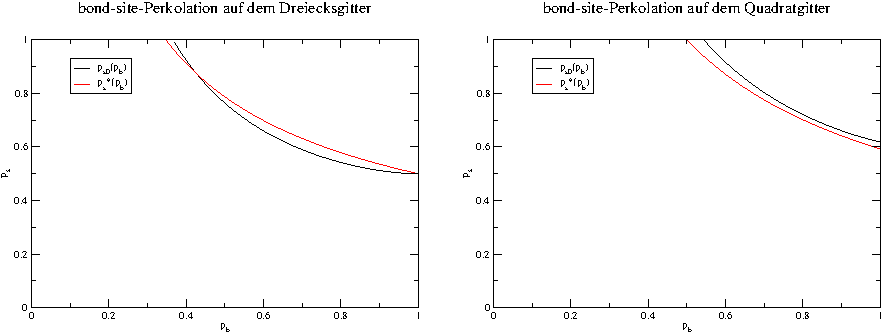
\includegraphics{./Schranken-figs/bond-site2d}
  \caption{$p_s^*(p_b)$ und $p_{s0}(p_b)$ ist links f\"ur das Dreiecks- und rechts f\"ur das Quadratgitter aufgetragen. F\"ur $p_s^*(p_b)$ ist die in \cite{Yanuka:90} vorgeschlagene Formel benutzt worden.}
  \label{fig:bond-site2d}
\end{figure}
\\In zwei Dimensionen wurde $\chi(p_s,p_b)$ f\"ur das Quadrat- (siehe Kap. \ref{sec:bondsitesq}) und das Dreiecksgitter (siehe Anhang \ref{sec:appbond-site}) ausgerechnet. Die Euler-Charakteristik der bond-site-Perkolation auf dem Dreiecksgitter ist
\begin{equation}
\chi^{tr}(p_s,p_b)=p_s-3p_bp_s^2+2p_b^3p_s^3.
\end{equation}
F\"ur das Quadratgitter erh\"alt man
\begin{equation}
\chi^{sq}(p_s,p_b)=p_s-2p_bp_s^2+p_b^4p_s^4.
\end{equation}
Aus der Gleichung $\chi(p_s,p_b)=0$ erh\"alt man eine Kurve $p_{s_0}(p_b)$ und kann diese mit $p^*_s\left(p^*_b\right)$ vergleichen. In beiden F\"allen hat $p_{s_0}(p_b)$ in etwa die gleiche Form wie die kritische Kurve, und beide Kurven liegen dicht zusammen (siehe Abb. \ref{fig:bond-site3d}). Beim Quadratgitter liegt die Nullstelle immer jenseits der Perkolationsschwelle, im Fall des Dreiecksgitters schneiden sich beide Kurven.
\\In drei Dimensionen wurde $\chi(p_s,p_b)$ f\"ur das fcc-Gitter (siehe Anhang \ref{sec:appbond-site}) und das sc-Gitter (siehe Kap. \ref{sec:bondsitesc}) ausgerechnet. 
\begin{equation}
 \chi^{fcc}(p_s,p_b)=p_s-6p_s^2p_b+8p_s^3p_b^3-2p_s^4p_b^6-p_s^6p_b^{12}.
\end{equation}
\begin{equation}
\chi^{sc}(p_s,p_b)= p_s-3p_s^2p_b+3p_s^4p_b^4-p_s^8p_b^{12}.
\end{equation}
Beim fcc- und sc-Gitter liegt $p_{s_0}(p_b)$ immer jenseits von $p_s^*(p_b^*)$, und beide Kurven haben fast identische Form (siehe Abb. \ref{fig:bond-site3d}).
\\

Auch bei bond-site-Perkolation best\"atigt sich die Beobachtung, dass die Nullstelle der Euler-Charakteristik in der N\"ahe der Perkolationsschwelle liegt. Beim zweidimensionalen Quadratgitter und bei den dreidimensionalen Gittern liegt die Nullstelle jenseits der Perkolationsschwelle, analog zu $p_c<p_0$ bei der reinen site-Perkolation. Neben den in Abschnitt \ref{sec:chibond} f\"ur bond-Perkolation auf archimedischen Gittern berechneten Euler-Charakteristiken, kann aus $\chi(p_s=1,p_b)$ eine weitere Euler-Charakteristik f\"ur bond-Perkolation erhalten werden. Die Nullstellen dieser Euler-Charakteristik liegt in allen F\"allen, anders als bei den Euler-Charakteristiken der \"Uberdeckungsgittern, \"uber der Perkolationsschwelle.

\begin{figure}[htbp]
  \centering
  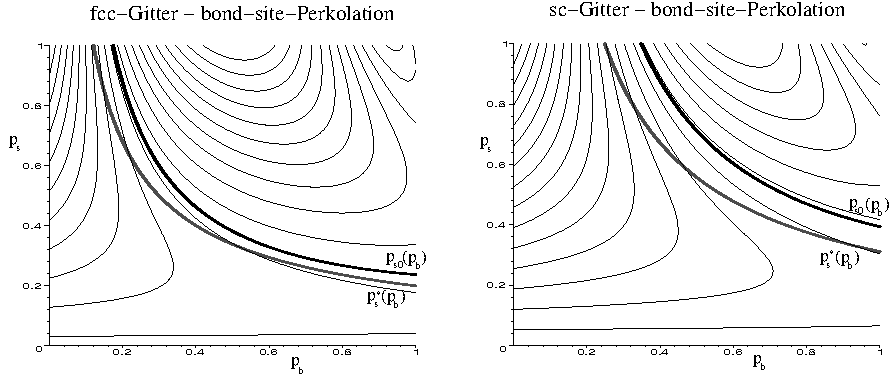
\includegraphics[height=20cm]{./Schranken-figs/bond-site3d}
  \caption{Die Kurven $p_s^*(p_b)$ und $p_{s_0}(p_b)$ haben sowohl f\"ur das fcc-, als auch f\"ur das sc-Gitter fast identische Form. Die d\"unnen Linien sind die H\"ohenlinien der $\chi(p_s,p_b)$-''Landschaft''. F\"ur $p_s^*(p_b)$ ist die in Ref. \cite{Yanuka:90} vorgeschlagene Formel benutzt worden.}
  \label{fig:bond-site3d}
\end{figure}